\documentclass[
	%parspace, % Add vertical space between paragraphs
	%noindent, % No indentation of first lines in each paragraph
	%nohyp, % No hyphenation of words
	%twoside, % Double sided format
	%draft, % Quicker draft compilation without rendering images
	%final, % Set final to hide todos
]{elteikthesis}[2023/04/10]

% The minted package is also supported for source highlighting
% See elteikthesis_minted.tex for example
%\usepackage[newfloat]{minted}

% Document's metadata
\title{Bejelentett illegális szemétlerakatok térképes vizualizációja} % title
\date{2024} % year of defense

% Author's metadata
\author{Kiszely Gergő János}
\degree{programtervező informatikus BSc}

% Superivsor(s)' metadata
\supervisor{Cserép Máté András} % internal supervisor's name
\affiliation{egyetemi tanársegéd} % internal supervisor's affiliation
%\extsupervisor{Külső Kornél} % external supervisor's name
%\extaffiliation{informatikai igazgató} % external supervisor's affiliation

% University's metadata
\university{Eötvös Loránd Tudományegyetem} % university's name
\faculty{Informatikai Kar} % faculty's name
\department{Programozáselmélet és Szoftvertechnológiai\\ Tanszék} % department's name
\city{Budapest} % city
\logo{elte_cimer_szines} % logo

% Add bibliography file
\addbibresource{elteikthesis.bib}

% The document
\begin{document}

% Set document language
\documentlang{hungarian}
%\documentlang{english}

% List of todos (not in the final document)
%\listoftodos[\todolabel]

% Title page (mandatory)
\maketitle
% Topic declaration page (mandatory) - can also be attached instead
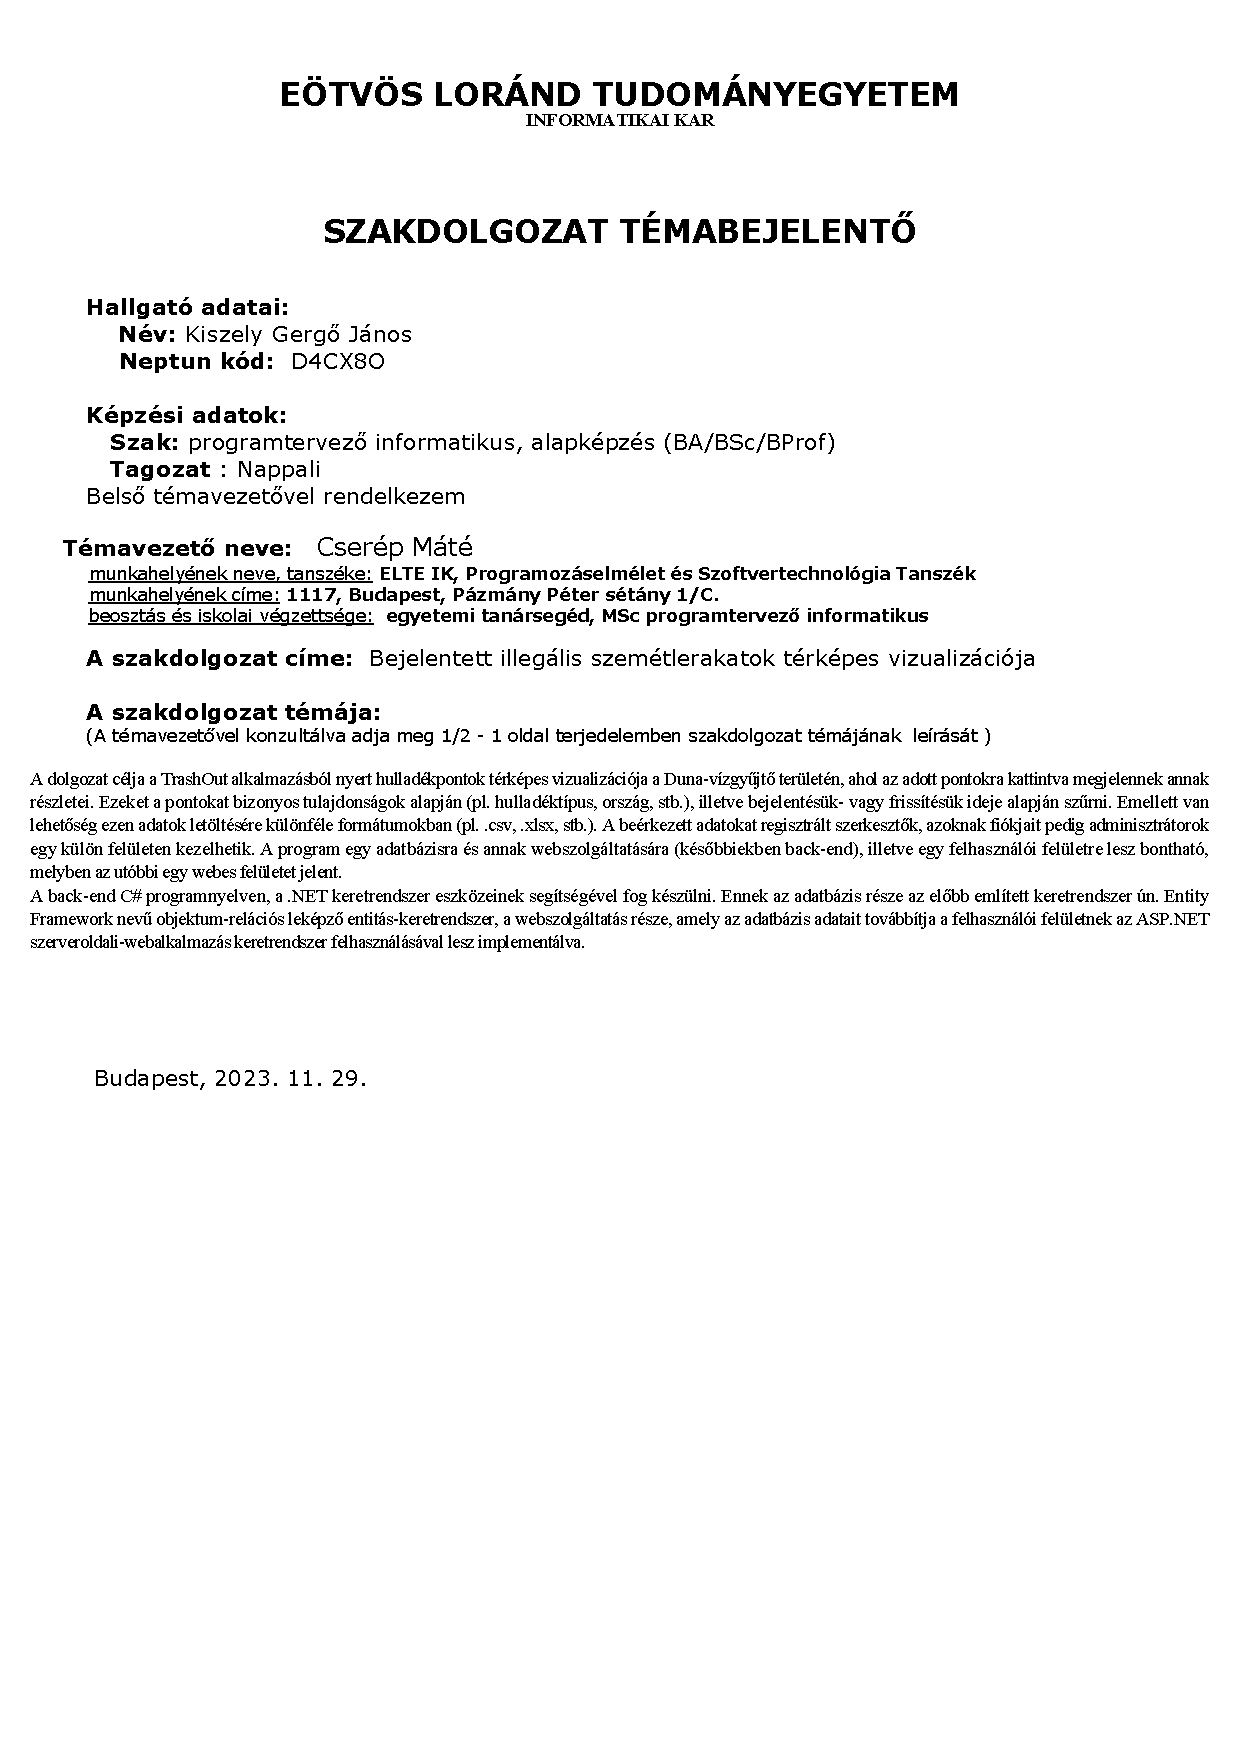
\includepdf{chapters/topic.pdf}

% Table of contents (mandatory)
\tableofcontents
\cleardoublepage

% Main content
\chapter{Bevezetés}
\label{ch:intro}

Az illegális szemétlerakatok jelensége modern világunkban egy súlyos probléma, amely nem csak környezetünket károsítja, hanem egészségünkre és közösségeink jólétére is kihathat. Ez a jelenség fokozottan megfigyelhető Magyarországon is, főként folyóink és tavaink, illetve településink határaiban. Ahogy világunk fejlődik és változik, úgy egyre több, ember által okozott szennyezéssel kell szembenéznünk azáltal, hogy megőrizzük környezetünk tisztaságát és egészségét. Habár ehhez az első lépés az emberek figyelmének felhívása, viszont a második mindenképpen a már természetbe jutott szemét mihamarabbi eltávolítása és nem utolsó sorban a környezet rehabilitálása.\par
Ezen dolgozatnak a célja is hasonló, amely az előbb említett illegális szemétlerakatok adatbázisba gyűjtése a lakosság segítségével, illetve annak térképes vizualizációja, mely segít azoknak a civil önkénteseknek, akik a környezetvédelem érdekében alkalmilag, vagy akár rendszeresen takarítják és szállítják el ezeket. Ehhez társul egy minimálisztikus közösségi médiához hasonló felület is, ahol minden regisztrált felhasználó a saját profilján gyűjtheti a már általa bejelentett pontokat. A célt és az implementációt a Tiszta Tisza Térkép ihlette, ahol a TrashOut nevű alkalmazásból nyert végpontokat tüntetik fel hasonlóan a weboldalukon, mely a weboldal tulajdonosai által évente megrendezett PET Kupa című hulladékgyűjtő verseny alkalmával használják azt lehetséges szemétlelőhelyek fellelésére. Míg az előbb említett oldalon csak a pontok megtekintésére van lehetőség, az előbb említett alkalmazásból kinyert adatokkal, addig ebben a programban lehetőség van jóváhagyásos regisztrálás után azok bejelentésére, illetve azok adatainak frissítésére/javítására is.
\newpage
\cleardoublepage

\chapter{Felhasználói dokumentáció}
\label{ch:user}

\section{Rendszerkövetelmények}

\subsection{Futtatás}

Magának webalkalmazás szerveroldalának a futtatásához a ASP.NET Core Runtime 8.0-ra van szükség, amelyhez
szükséges az alábbi operációs rendszerek valamelyike:
\begin{compactitem}
	\item Windows 10, 11 vagy Server 2012+
	\item 64-bites Ubuntu 20.04+ vagy Debian 11+
	\item macOS 10.15+ (csak külső, hosztolt szerver esetén támogatott)
\end{compactitem} 
A memóriahasználat a felhasználóktól nagyban függ, így 0,5 GB-tól akár 4 GB RAM-ra is szüksége lehet a szervernek a zökkenőmentes futáshoz. A merevlemezen történő tárhelyhasználat nagyban függ az éppen bejelentett pontok méretétől és legfőképp az azokhoz csatolt fényképektől. Magához a futtatáshoz elegendő 0,5 GB tárhely is (az ehhez szükséges szoftvereket nem bele értve), viszont az alkalmazás használtat közben ez nagy mértékben fog növekedni az előbb említett okok miatt, így érdemes akár saját, nagy kapacitású merevlemezre telepíteni a szerveroldalt.
Az szerver által használt SQL Server adatbázishoz (későbbiekben MSSQL-adatbázis) a Microsoft SQL Server szoftver valamelyik, de lehetőség szerint a legfrissebb, 2019-es verziójára van szükség, melyet a fentebb említett operációs rendszerek bármelyike képes futtatni.
Az első üzembe helyezést követően nincsen szükség további rendszergazdai feladatokra.
\subsection{Használat}

A program felhasználói felülete egy weboldal. Ennek meglátogatásához elsősorban szükség van egy olyan operációs rendszer telepítésére, majd futtatására, melyre elérhető bármilyen friss, Chromium-alapú webböngésző. Egy ilyen böngésző a Google Chrome, amellyel ajánlott a weboldal látogatása. Hardver- és szoftver követelményei az alábbiak:
\begin{compactitem}
	\item Operációs rendszerek valamelyike:
	\begin{compactitem}
		\item Windows 10, 11 vagy Server 2012+
		\item 64-bites Ubuntu 20.04+ vagy Debian 11+
		\item macOS 10.15+
		\item Android 8.0+ vagy Chrome OS
	\end{compactitem}
	\item Minimális hardver követelmények:
	\begin{compactitem}
		\item Pentium 4+ (vagy más, SSE3-at támogató) processzor
		\item 2 (ajánlottan 4) GB RAM
	\end{compactitem}
\end{compactitem}

Felhasználóként első üzembe helyezésre nincsen szükség, elég ha a felhasználó meglátogatja az oldalt. Ha még nem regisztrált felhasználói fiókot, akkor bizonyos funkciók eléréséhez regisztrálnia kell.

\section{Általános felhasználói tájékoztató}

Az weboldal használtat közben négy felhasználói típusról beszélhetünk: vendég, regisztrált (és bejelentkezett) felhasználó, moderátor és adminisztrátor. Így vendégnek számít aki még nem regisztrált, vagy ha igen, akkor nem jelentkezett be fiókjával, moderátornak aki moderátori szintű fiókkal és adminisztrátornak, aki adminisztrátori szintű fiókkal azonosította magát a bejelentkező felületen.
\newpage

\section{Funkciók vendégként}

\noindent Egy vendég felhasználó számára hat funkció érhető el a weboldalon:
\begin{compactitem}
	\item regisztrálás új-, illetve bejelentkezés már meglévő fiókba
	\item a térkép megtekintése a bejelentett pontokkal (ez a főoldal)
	\item egy-egy pont adatainak részletesebb megtekintése
	\item az összes pont listázása
	\item a weboldal színsémájának ("sötét"- vagy "világos" mód) tetszőleges beállítása
\end{compactitem}

\begin{figure}[H]
	\centering
	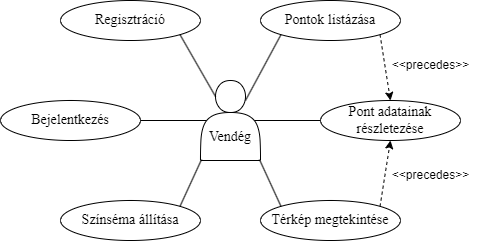
\includegraphics[width=0.6\textwidth]{usecase_guest}
	\caption{Felhasználói esetek vendégként}
	\label{fig:usecase_guest}
\end{figure}

\subsection{Felület áttekintése}
\label{subsec:nav_guest}

A weboldal látogatása során több felület is megjelenik, viszont ezek általánosan leírhatóak. Minden lap tetején egy navigációs sáv van, melynek segítségével több funkciót is gyorsan elérhetünk. A sáv bal oldalán a weboldal neve, illetve a "Térkép" felirat egyaránt a térképre, azaz a főoldalra irányít, a mellette szereplő "Lista" pedig a pontok listájához. A másik oldalon (jobbról balra) egy fizikai kapcsolót imitáló gomb, melynek segítségével válthatunk az előbb említett színsémák között, illetve amellett egy "Nincs bejelentkezve" feliratú listát lenyitva tudunk a regisztráció, illetve a bejelentkezés közül választani.\par
Ha a felhasználó nem egy széles képernyőn (pl. asztali számítógép vagy fektetett táblagép) látogatja meg az oldalt, akkor a sáv bár hasonlóan ott van, viszont a könnyebb használat érdekében a menüpontok egy, a jobb oldalon található \hspace{0.1cm}\boldmath\(\equiv\)\hspace{0.1cm} ikonra kattintva lehet ezeket elérni.

\begin{figure}[H]
	\centering
	\subcaptionbox{Nagy méretű kijelző}{
		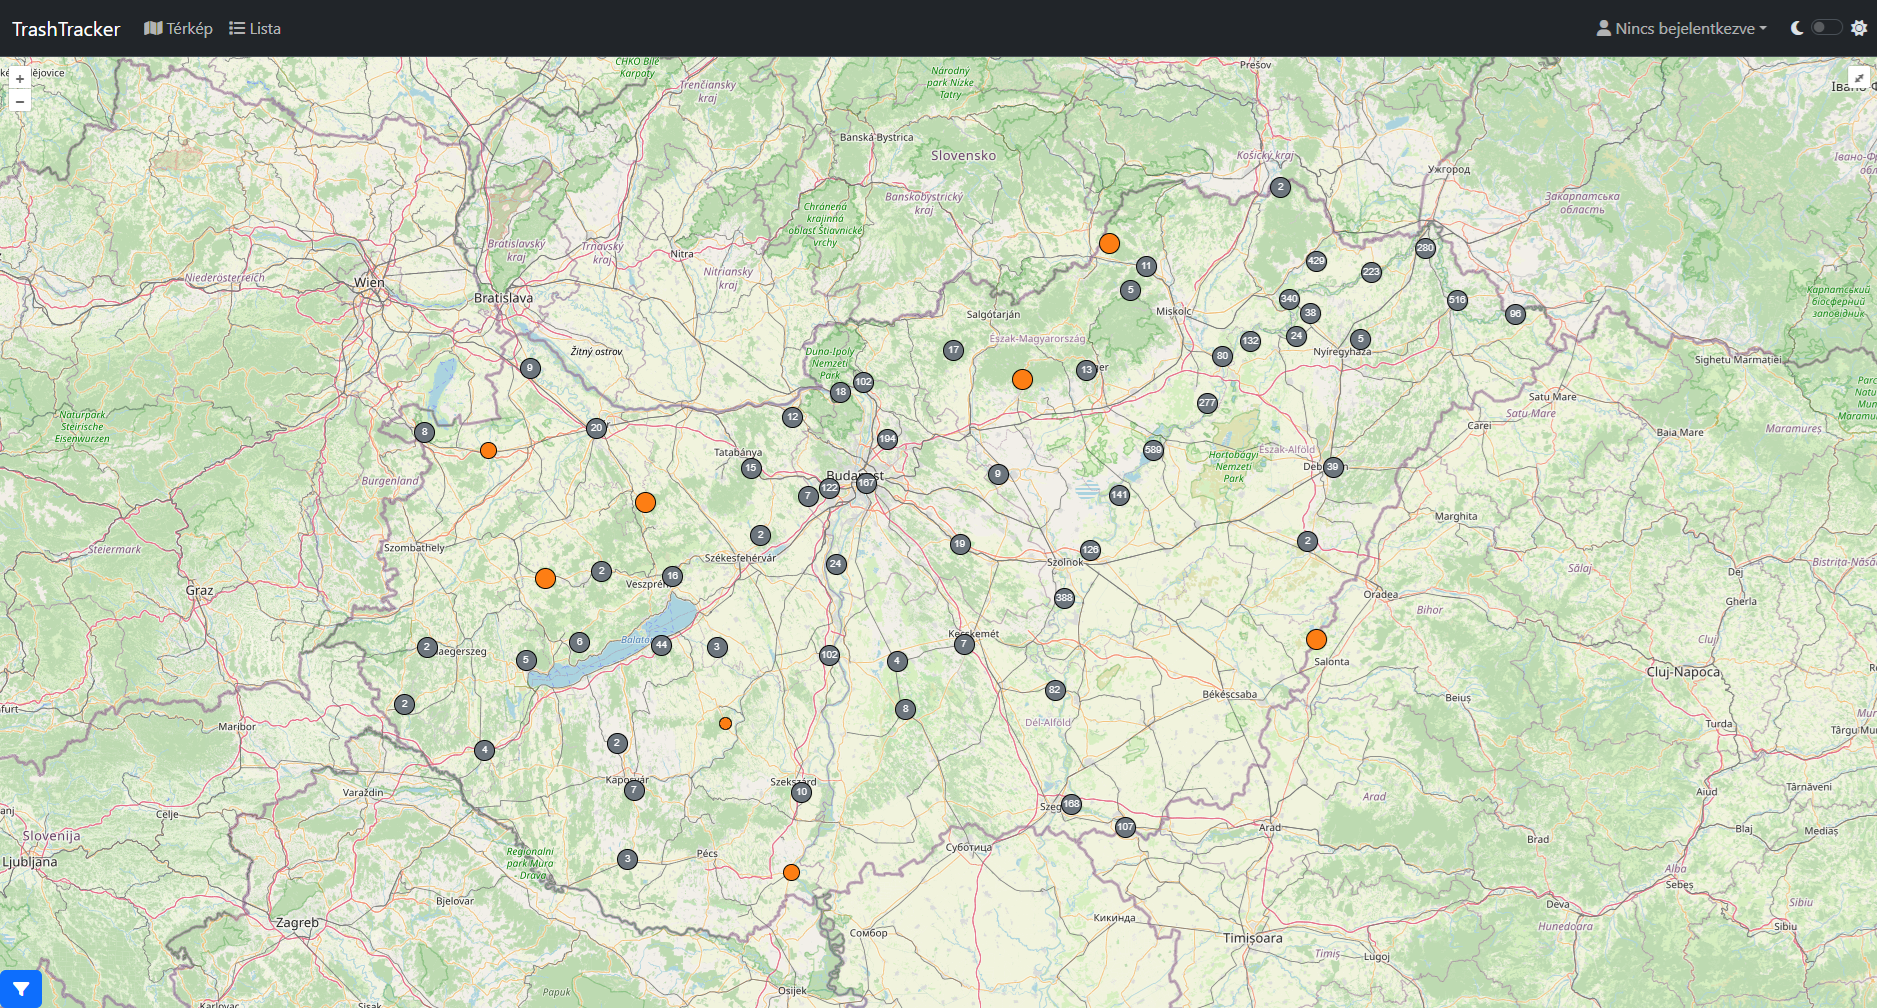
\includegraphics[width=0.7\linewidth]{map}}
	\hspace{5pt}
	\subcaptionbox{Kis méretű kijelző}{
		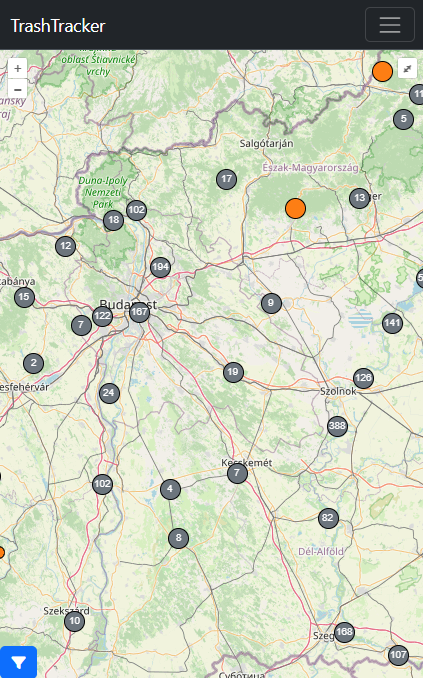
\includegraphics[width=0.3\linewidth]{map_phone}}
		\hspace{5pt}
	\subcaptionbox{Kis méretű kijelző (lenyitott navigációs sávval)}{
		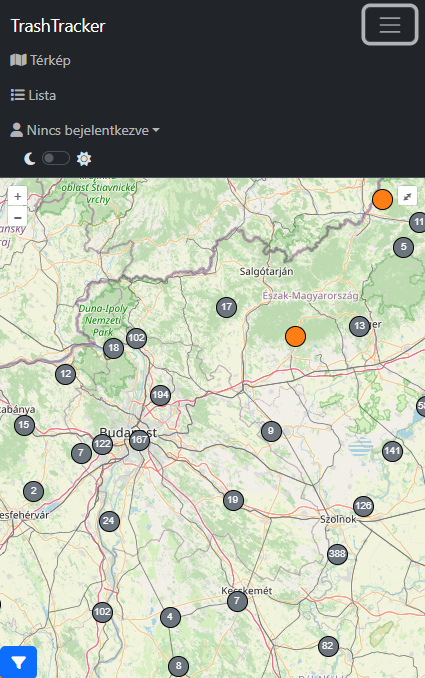
\includegraphics[width=0.3\linewidth]{map_phone_menu}}
	\caption{A felület kinézete a kezdőoldalon különböző méretű kijelzők esetén}
	\label{fig:map_guest}
\end{figure}

\subsection{Térkép (kezdőoldal)}
\label{subsec:map_guest}

A navigációs sávon a weboldal nevére, illetve a "Térkép" feliratra kattintva azonnal a bejelentett pontok térképére navigálhatunk. Ennek kezelése a már jól ismert térképes alkalmazásokéhoz hasonló. A bal felső sarokban található \hspace{0.1cm}\boldmath\(+\)\hspace{0.1cm}, illetve \hspace{0.1cm}\boldmath\(-\)\hspace{0.1cm} ikonra kattintva nagyítani, illetve kicsinyíteni lehet, emellett egérrel a görgő görgetésével és érintőképernyőn két ujj összehúzásával/széttolásával is lehetőség van. A jobb felső sarokban a térképet teljes képernyős módba is lehet helyezni, melynek ismételt megnyomásával, vagy billentyűzeten az Esc gombbal ki lehet lépni. A bal alsó sarokban található a szűrés gomb, melynek segítségével különböző, a felhasználók által jelentett tulajdonságok szerint van lehetőség.

\subsubsection{Jelmagyarázat}

A térképen a pontok különböző mérettel és színnel jelennek meg, melyeknek céljuk a fontosabb információk lehetőség szerinti kiemelése.\\
A szemét mennyisége szerint a pont mérete lehet
\begin{compactitem}
	\item[\large\textbullet] kicsi (8 pixel), azaz "elfér egy zsákban",
	\item[\Large\textbullet] közepes (10 pixel), azaz "elfér egy talicskában" és
	\item[\LARGE\textbullet] nagy (12 pixel), azaz "autóra van szükség".
\end{compactitem}
A szemét első bejelentés óta levő állapota szerint a pont színe lehet
\begin{compactitem}
	\item[\textcolor{tt_green}{\Large\textbullet}] zöld, azaz "megtisztítva",
	\item[\textcolor{tt_yellow}{\Large\textbullet}] sárga, azaz "kevesebb",
	\item[\textcolor{tt_orange}{\Large\textbullet}] narancs, azaz "még mindig itt van" és
	\item[\textcolor{tt_red}{\Large\textbullet}] piros, azaz "több".
\end{compactitem}

\subsubsection{Szűrés}

A fentebb említett szűrés gombra kattintva a képernyő alján beúszik egy görgethető menü, amely a pontok tulajdonságai szerinti szűrést teszi lehetővé. A szemét mennyisége és állapota mellett annak típusa és hozzáférhetősége szerint is lehet válogatni. Ezeket a beúszó menün található, tulajdonságok szerint csoportosított "kapcsoló" gombokkal lehet elérni. Ha egy ilyen gomb kék színű, akkor igen, ha átlátszó, akkor pedig nem szeretnénk a térképen látni. Alapértelmezetten az összes ilyen gomb "igen" állapotban van. A gombok között szűrés esetén a logikai vagy művelete értelmezett, tehát ha bejelölésre kerül egy tulajdonság, viszont egy másik nem, akkor attól függetlenül a bejelöletlen attribútum még előfordulhat a megjelenített pontok között, feltéve, hogy legalább egy bejelölt jellemzővel rendelkezik. Ezt a menüt a jobb felső sarokban található \hspace{0.1cm}\boldmath\(\times\)\hspace{0.1cm} gombra nyomva lehet bezárni, a szűrőket megtartva, egy másik oldalra navigálásig vagy az oldal újratöltéséig.

\begin{figure}[H]
	\centering
	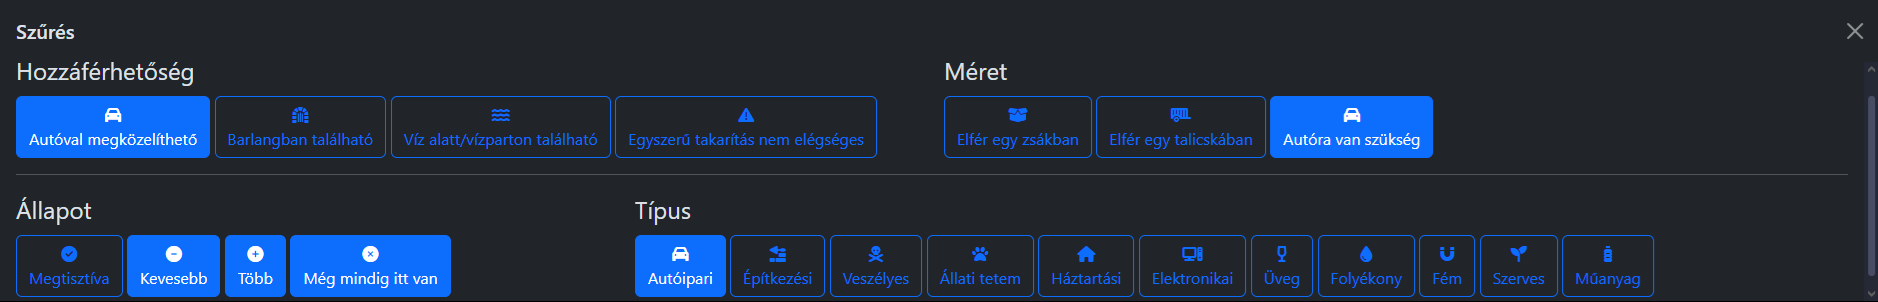
\includegraphics[width=1\textwidth]{map_filter}
	\caption{A kezdőoldal alján beúszó szűrési menü}
	\label{fig:map_filter}
\end{figure}

\subsubsection{Pontok letöltése}

A térképen szereplő bejelentett pontok letöltésére is van lehetőség .csv formátumban. Ehhez a térkép jobb alsó sarkában található \hspace{0.1cm}\faIcon{download}\hspace{0.1cm} ikonnal ellátott zöld gombra kell kattintani, mellyel automatikusan elindul a fájl letöltése. Ez a vesszővel elválasztott formátum könnyen importálható táblázatkezelő szoftverekbe, illetve egyszerűen felhasználható külön, a fájl feldolgozására implementált programokban is.

\subsubsection{Betekintés és részletek}

Egy pontra való kattintáskor afelett megjelenik egy modális "buborék", amely minimális információt és egy képet tartalmaz a hozzátartozó szemétről. Emellett a kis ablak alján található egy "Részletek" gomb, melyre kattintva elnavigálhatunk az azt részletező adatlapra.

\begin{figure}[H]
	\centering
	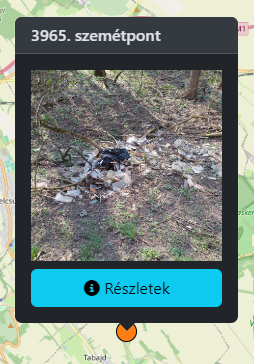
\includegraphics[width=0.225\textwidth]{map_popover}
	\caption{Példa egy felbukkanó buborékra egy ponton}
	\label{fig:map_popover}
\end{figure}

\subsection{Pont részletezése}
\label{subsec:trash_details}

Ezt az oldalt az előző bekezdésben említett "Részletek" gombra kattintva, vagy a következő bekezdésben tárgyalt \faIcon{info-circle} ikonra kattintva lehet elérni. Itt az egyszerű tulajdonságok részletezésén túl megtalálható a pont pontos helyzete, illetve annak forrása (felhasználó esetén bejelentője). Előbbire kattintva a térképen levő helyére, utóbbira pedig annak forrására (TrashOut esetén az ottani adatlapjára, felhasználó esetén annak a profiljára) lehet navigálni.

\begin{figure}[H]
	\centering
	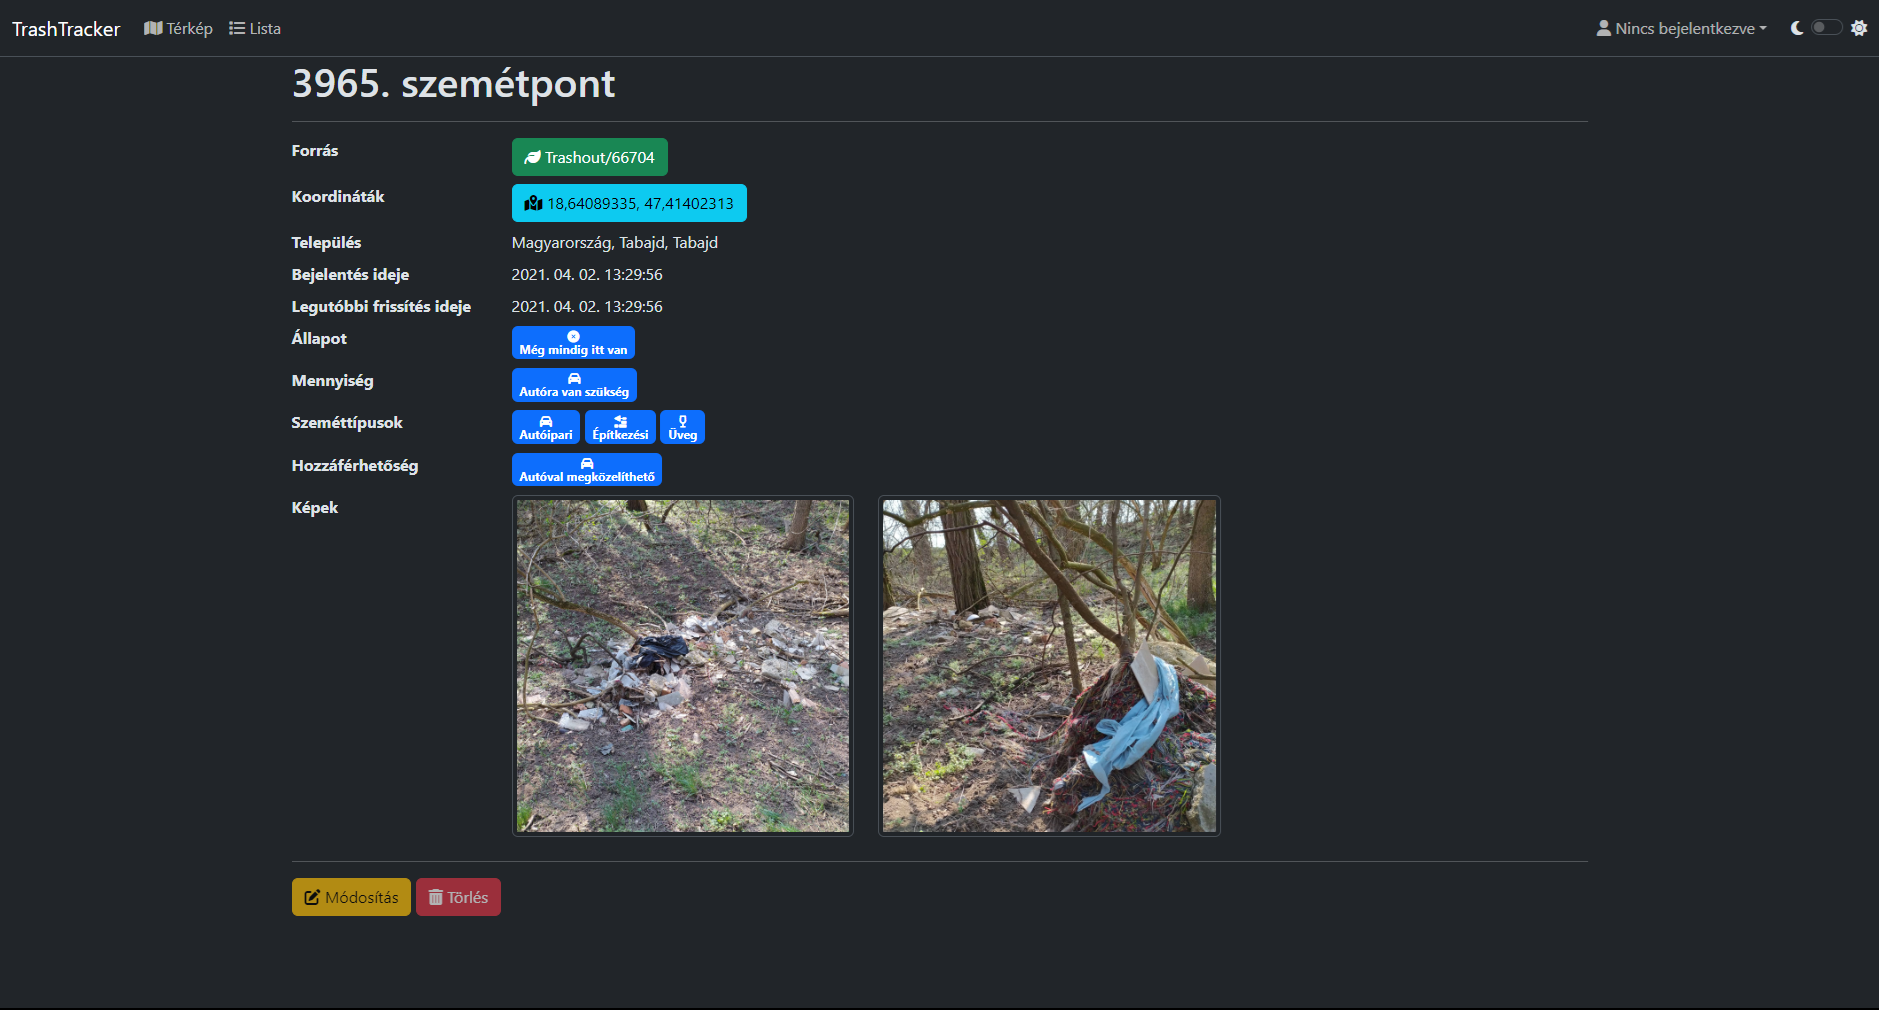
\includegraphics[width=0.7\textwidth]{trash_details}
	\caption{Példa egy szemétpontot részletező adatlapra}
	\label{fig:trash_details}
\end{figure}

\subsection{Listanézet}
\label{subsec:trash_index}

A pontokat nem csak térképen, hanem listaként is megtekinthetjük. Ennek célja, hogy a bejelentés/frissítés dátuma szerint rendezve könnyedén fel lehessen fedezni a legrelevánsabb szemétlerakatokat. A lista minden sora egy-egy pontot, annak oszlopai pedig annak a fejlécben szereplő tulajdonságát tartalmazzák. Egy adott rekord részletezésére is lehetőség van, a jobb oldalon található \faIcon{info-circle} ikonra kattintva. Az oldal tetején lehetőség van alapvető szűrésekre is, opcionálisan belefoghatjuk a listába a már megtisztított pontokat, kereshetünk a bejelentő felhasználónevében, illetve az ahhoz tartozó megjegyzéseiben, illetve állíthatjuk az egy oldalon szereplő találatok maximális számát. Ha több találat van, mint ami az oldalon elfér, akkor a lista tetején, illetve alján található nyilakkal és számokkal könnyedén navigálhatunk azok között.

\begin{figure}[H]
	\centering
	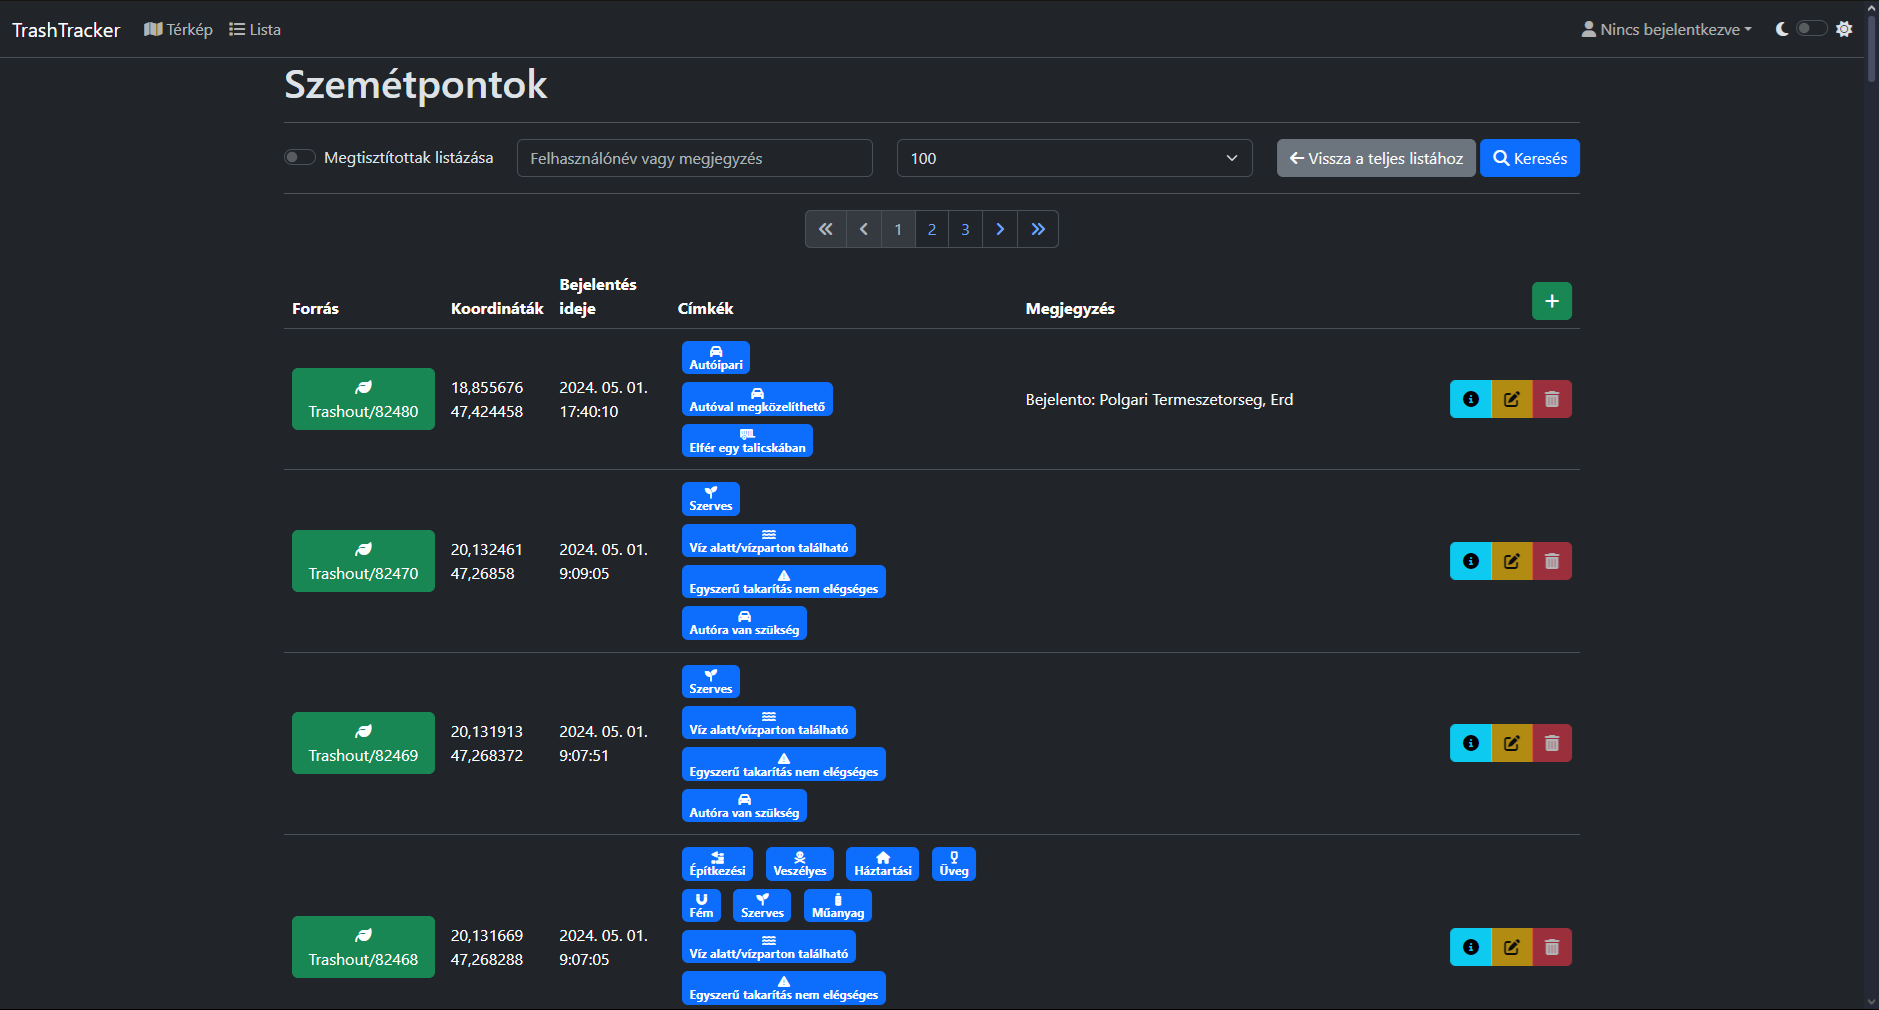
\includegraphics[width=0.7\textwidth]{trash_index}
	\caption{Szemétpontok listanézetének felülete}
	\label{fig:trash_index}
\end{figure}

\subsection{Színséma választása}

Minden oldal navigációs sávjának jobb szélén található egy kapcsoló mellyel könnyedén állítható az adott oldal színsémája, melynek bal- (\faIcon{moon}) állása sötét, illetve jobb oldali (\faIcon{sun}) állása világos módot jelent. Alapértelmezetten ez az előbbi állapotban van az energiatakarékosabb működés és a szemet jobban kímélő megjelenés miatt. Ez a beállítás szabadon állítható, mely megmarad minden aloldalon a böngészés idejére.

\begin{figure}[H]
	\centering
	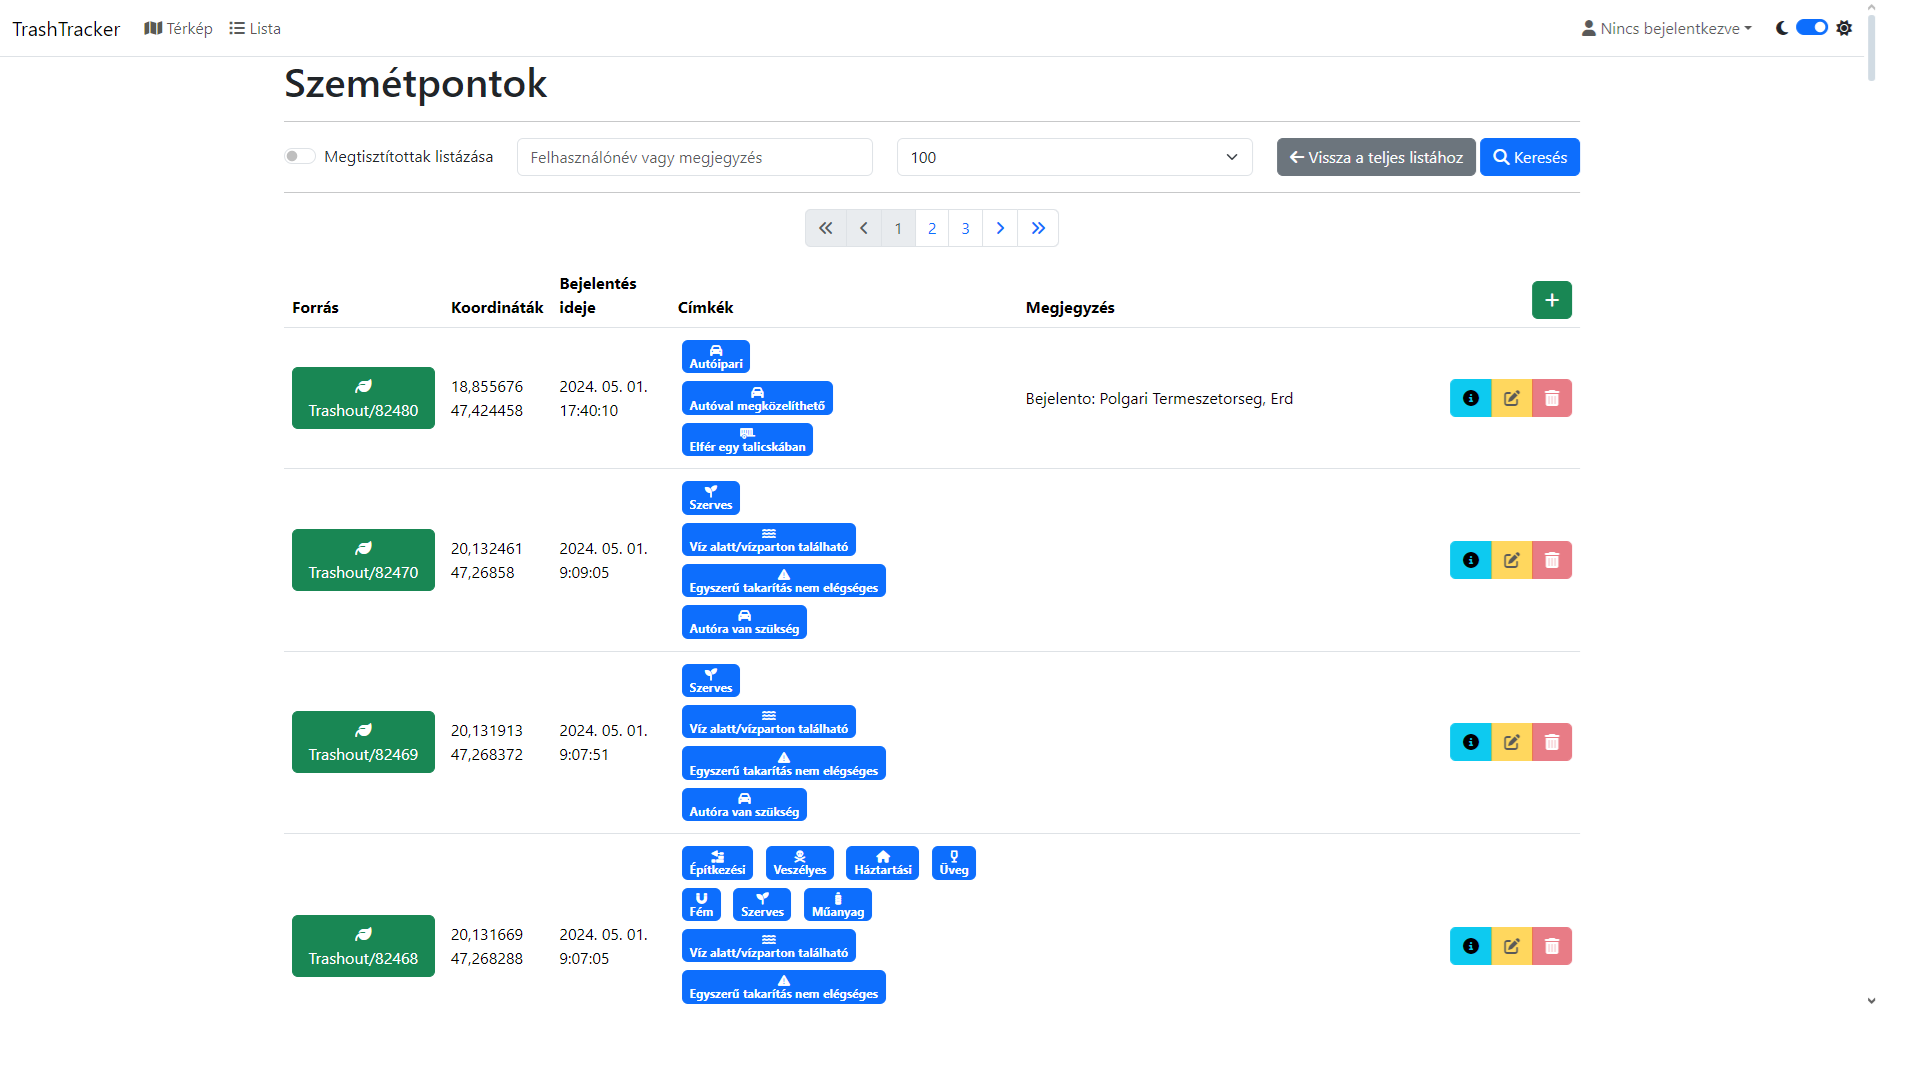
\includegraphics[width=0.7\textwidth]{trash_index_light}
	\caption{Szemétpontok listanézetének felülete világos módban}
	\label{fig:trash_index_light}
\end{figure}

\subsection{Regisztráció}
\label{subsec:register}

További funkciók használatáért (pontok bejelentése és frissítése) a felhasználónak egy felhasználói fiókra van szüksége, mely utóbbija ha nincs, akkor regisztrálnia kell hozzá. Ezt a navigációs sáv jobb oldalán található "Nincs bejelentkezve" feliratra kattintva lenyíló menüben szereplő "Regisztráció" menüpontra nyomva érheti el. Ha az előbbi helyett egy \faIcon{user} ikonnal társulva egy felhasználó neve szerepel, akkor az már be van jelentkezve, ezzel kapcsolatosan nincsen teendője.\par
A regisztrációs felületen egy űrlap található, ahol meg kell adni a kívánt felhasználónevet, e-mail címet (elérhetőségként), jelszavat, illetve opcionálisan egy profilképet. Az adatok kitöltése után az űrlap alján található "Regisztráció" gombra kattintva lehet beadni az adatokat, melyek ha megfelelnek a követelményeknek, akkor a felhasználó a főoldalon találja magát, az új fiókjával bejelentkezve.

\begin{figure}[H]
	\centering
	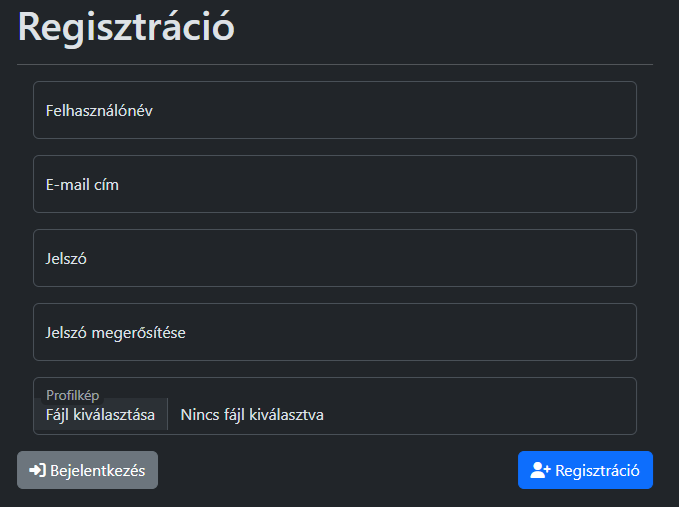
\includegraphics[width=0.7\textwidth]{register_form}
	\caption{A regisztrációs felület űrlapja}
	\label{fig:register_form}
\end{figure}

\subsubsection{Hibaüzenetek}
\label{subsubsec:user_register_errors}

A regisztrációkor megadott adatok több követelménynek is meg kell hogy feleljenek, melyek "megsértésekor" hibaüzenetek jelenhetnek meg az űrlap kitöltése közben vagy után. Az első ilyen követelmény, hogy minden felhasználónévnek egyedinek kell lennie. Ezt az űrlap helyes kitöltése és elküldése után egy "\textit{Ez a felhasználónév már foglalt!}" felirat jelzi.

\begin{figure}[H]
	\centering
	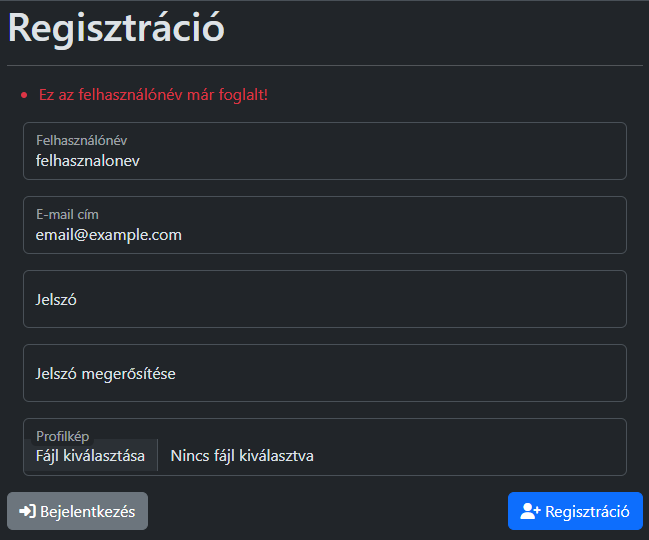
\includegraphics[width=0.7\textwidth]{register_form_duplicate_username}
	\caption{Már foglalt felhasználónév esetén megjelenő hibaüzenet}
	\label{fig:register_form_duplicate_username}
\end{figure}

Ha a megadott e-mail cím nem érvényes (azaz nem felel meg annak formai követelményeihez, pl. legyen benne "@" és egy "."), azt az űrlap kitöltése közben jelzi egy "\textit{Érvénytelen e-mail cím!}" feliratú üzenet.

\begin{figure}[H]
	\centering
	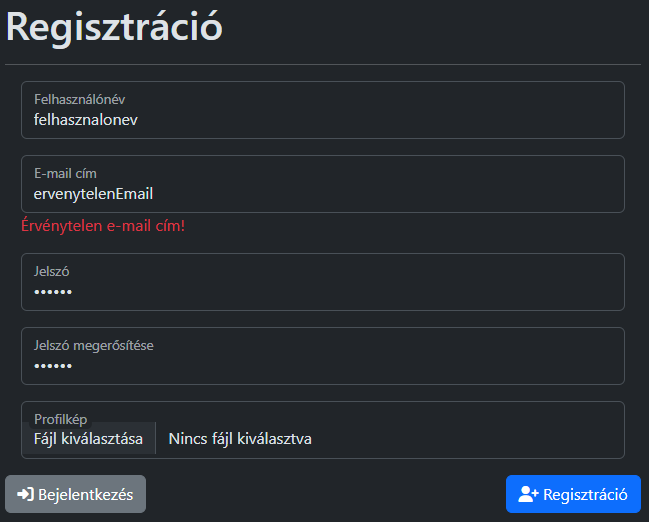
\includegraphics[width=0.7\textwidth]{register_form_invalid_email}
	\caption{Érvénytelen e-mail cím esetén megjelenő hibaüzenet}
	\label{fig:register_form_invalid_email}
\end{figure}

A legtöbb követelmény a jelszavakat érinti, itt több hibaüzenettel is találkozhat a felhasználó. Biztonsági okokból, egy jelszó 6-32 db karakterből kell álljon, melynek tartalmaznia kell legalább egy-egy kis- és nagybetűt, illetve számjegyet is. Ha ennek mégsem felelne meg a megadott jelszó, akkor azt az e-mail címhez hasonlóan egy "\textit{A jelszó nem lehet rövidebb 6 és hosszabb 32 karakternél!}" vagy "\textit{Jelszónak tartalmaznia kell legalább egy kis- és nagybetűt illetve számjegyet!}" üzenet jelenik meg, annak függvényében, hogy melyik pontján nem megy át az ellenőrzésen (tehát ha túl rövid a jelszó és pl. nem tartalmaz nagybetűt, akkor csak az előbbi jelenik meg, az utóbbi csak ha a hossz javítása után sem felel meg). Emellett a jelszó megerősítésére is szükség van, azaz meg kell adni a beírt jelszót egy második alkalommal is. Ha ezek nem egyeznének meg, azt is egy hibaüzenet jelzi a felhasználó számára.

\begin{figure}[H]
	\centering
	\subcaptionbox{Nem megfelelő hosszú jelszó hibaüzenete}{
		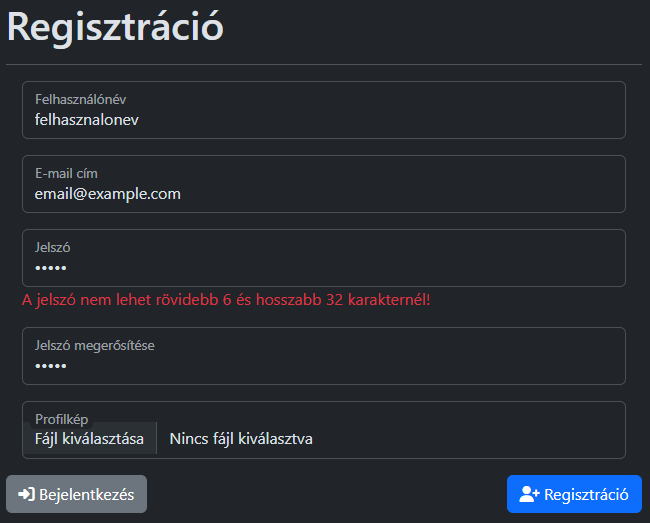
\includegraphics[width=0.3\linewidth]{register_form_invalid_password_length}}
	\hspace{5pt}
	\subcaptionbox{Nem megfelelő karaktereket tartalmazó jelszó hibaüzenete}{
		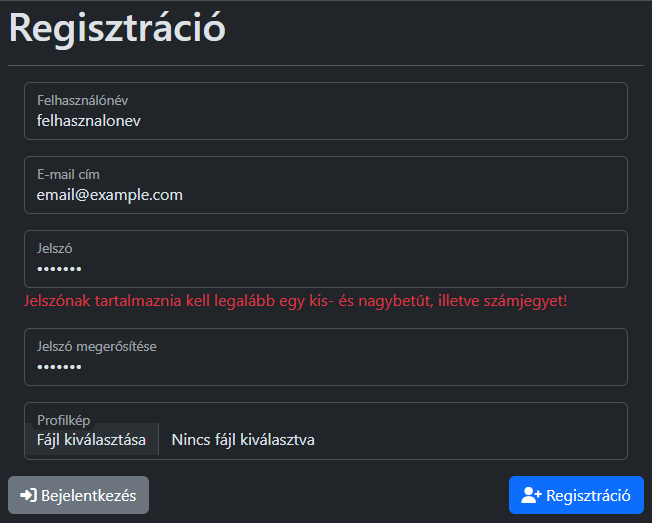
\includegraphics[width=0.3\linewidth]{register_form_invalid_password_characters}}
	\hspace{5pt}
	\subcaptionbox{Nem azonos jelszavak hibaüzenete}{
		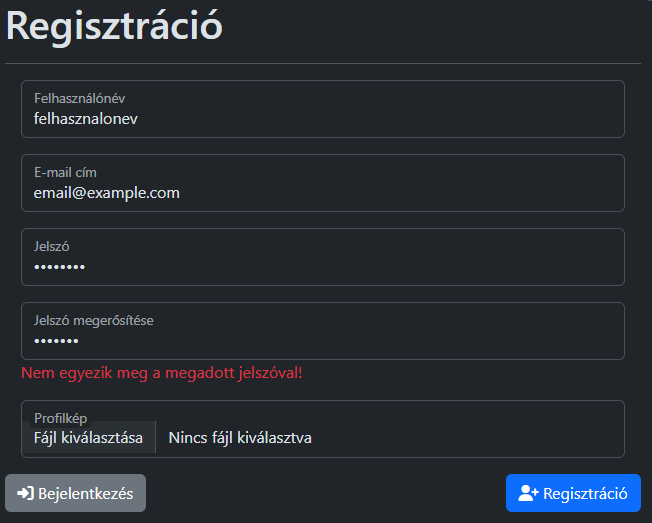
\includegraphics[width=0.3\linewidth]{register_form_invalid_password_repeat}}
	\caption{Érvénytelen jelszó esetén megjelenő hibaüzenetek}
	\label{fig:register_form_invalid_password}
\end{figure}

\subsection{Bejelentkezés}
\label{subsec:login}

Ha a felhasználónak már van saját fiókja, akkor ismételt regisztráció helyett beléphet abba, az előző bekezdésben tárgyaltak szerint a "Bejelentkezés" gombra kattintva. Az űrlap hasonló, viszont itt elég csak a felhasználónév (vagy e-mail cím tetszőlegesen), illetve a hozzátartozó jelszó egyszeri megadására. Ha az adatok egyeznek a regisztrációkor megadottakkal, akkor az űrlap alján található "Bejelentkezés" gombra kattintva a felhasználó a főoldalra lesz átirányítva, a felhasználói fiókjába bejelentkezve. Ellenben, ha nem jár sikerrel, akkor üzenetek tájékoztatják a klienst erről. Ha többszöri próbálkozásra sem jár sikerrel, akkor lehetősége van bejelentkezés helyett újabb felhasználó regisztrálására, vagy egy adminisztrátort megkérve bejelentkezési adatainak megváltoztatására is.

\begin{figure}[H]
	\centering
	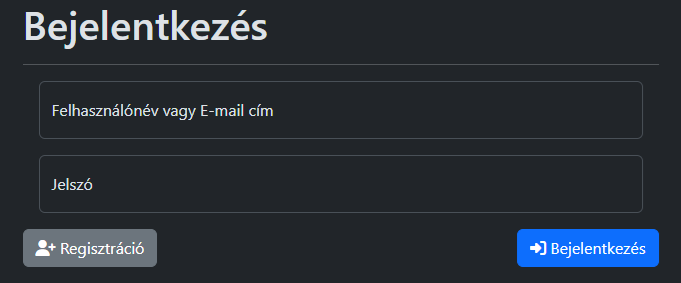
\includegraphics[width=0.7\textwidth]{login_form}
	\caption{A bejelentkezéses felület űrlapja}
	\label{fig:login_form}
\end{figure}

\subsubsection{Hibaüzenetek}

Sikertelen bejelentkezés esetén, azaz nem megfelelő felhasználónév (vagy e-mail cím) és jelszó páros megadásakor biztonsági okok miatt csak egy, a regisztráláskor látottaknál általánosabb "\textit{Sikertelen bejelentkezés!}" felirat szerepel.

\begin{figure}[H]
	\centering
	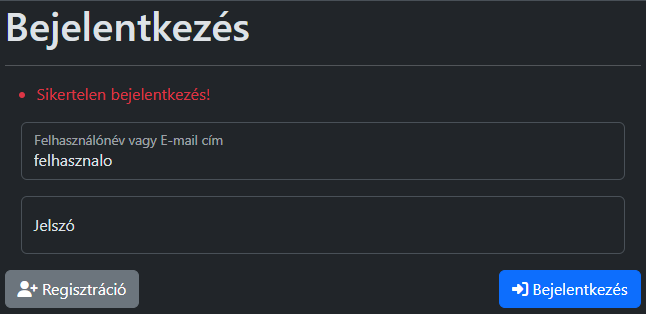
\includegraphics[width=0.7\textwidth]{login_form_error}
	\caption{A bejelentkezéses felület űrlapján szereplő hibaüzenet}
	\label{fig:login_form_error}
\end{figure}

\section{Funkciók felhasználóként}

Sikeres bejelentkezést (vagy regisztrációt) követően a felhasználó vendég helyett bejelentkezett felhasználónak (vagy fióktípusának megfelelőnek) számít. Ezzel további funkciók válnak elérhetővé, mint például a szemétpontok bejelentése és frissítése, illetve a saját felhasználói fiók profiljának szerkesztése.

\begin{figure}[H]
	\centering
	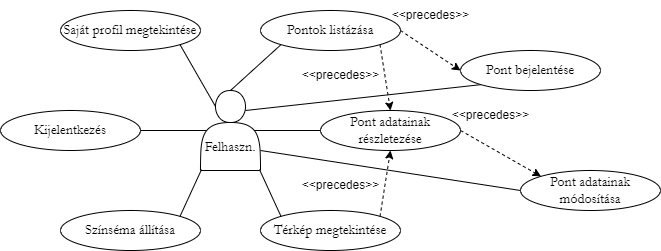
\includegraphics[width=1.0\textwidth]{usecase_user}
	\caption{Felhasználói esetek (bejelentkezett) felhasználóként}
	\label{fig:usecase_user}
\end{figure}

\subsection{Pont bejelentése}
\label{subsec:trash_create}

Új pont bejelentésére a listanézet tetején található \faIcon{plus} ikonra kattintva van lehetőség, mely elnavigál annak az űrlapjára. Ezen az űrlapon meg kell adni a szemét pontos helyzetét koordinátákként, amely megadásának segítségül szolgál a szöveges mezőjük melletti "Jelenlegi hely meghatározása", mely megnyomásával a böngésző meghatározza a bejelentőnek a lehető legpontosabb koordinátáit. A méret jellemzése mellett ajánlott a szemét típusát és hozzáférhetőségét is megadni, melynek kezelése hasonló a térképen való szűrés gombjaihoz. Az utolsó, többsoros szöveges mezőben megjegyzést lehet írni, mely segíti a listanézetben való keresését a pontnak. Az űrlap alján a "Vissza" gombbal lehet az előbb meglátogatott oldalra navigálni, illetve a "Bejelentés" gombra kattintva is ide lesz átirányítva a felhasználó

\begin{figure}[H]
	\centering
	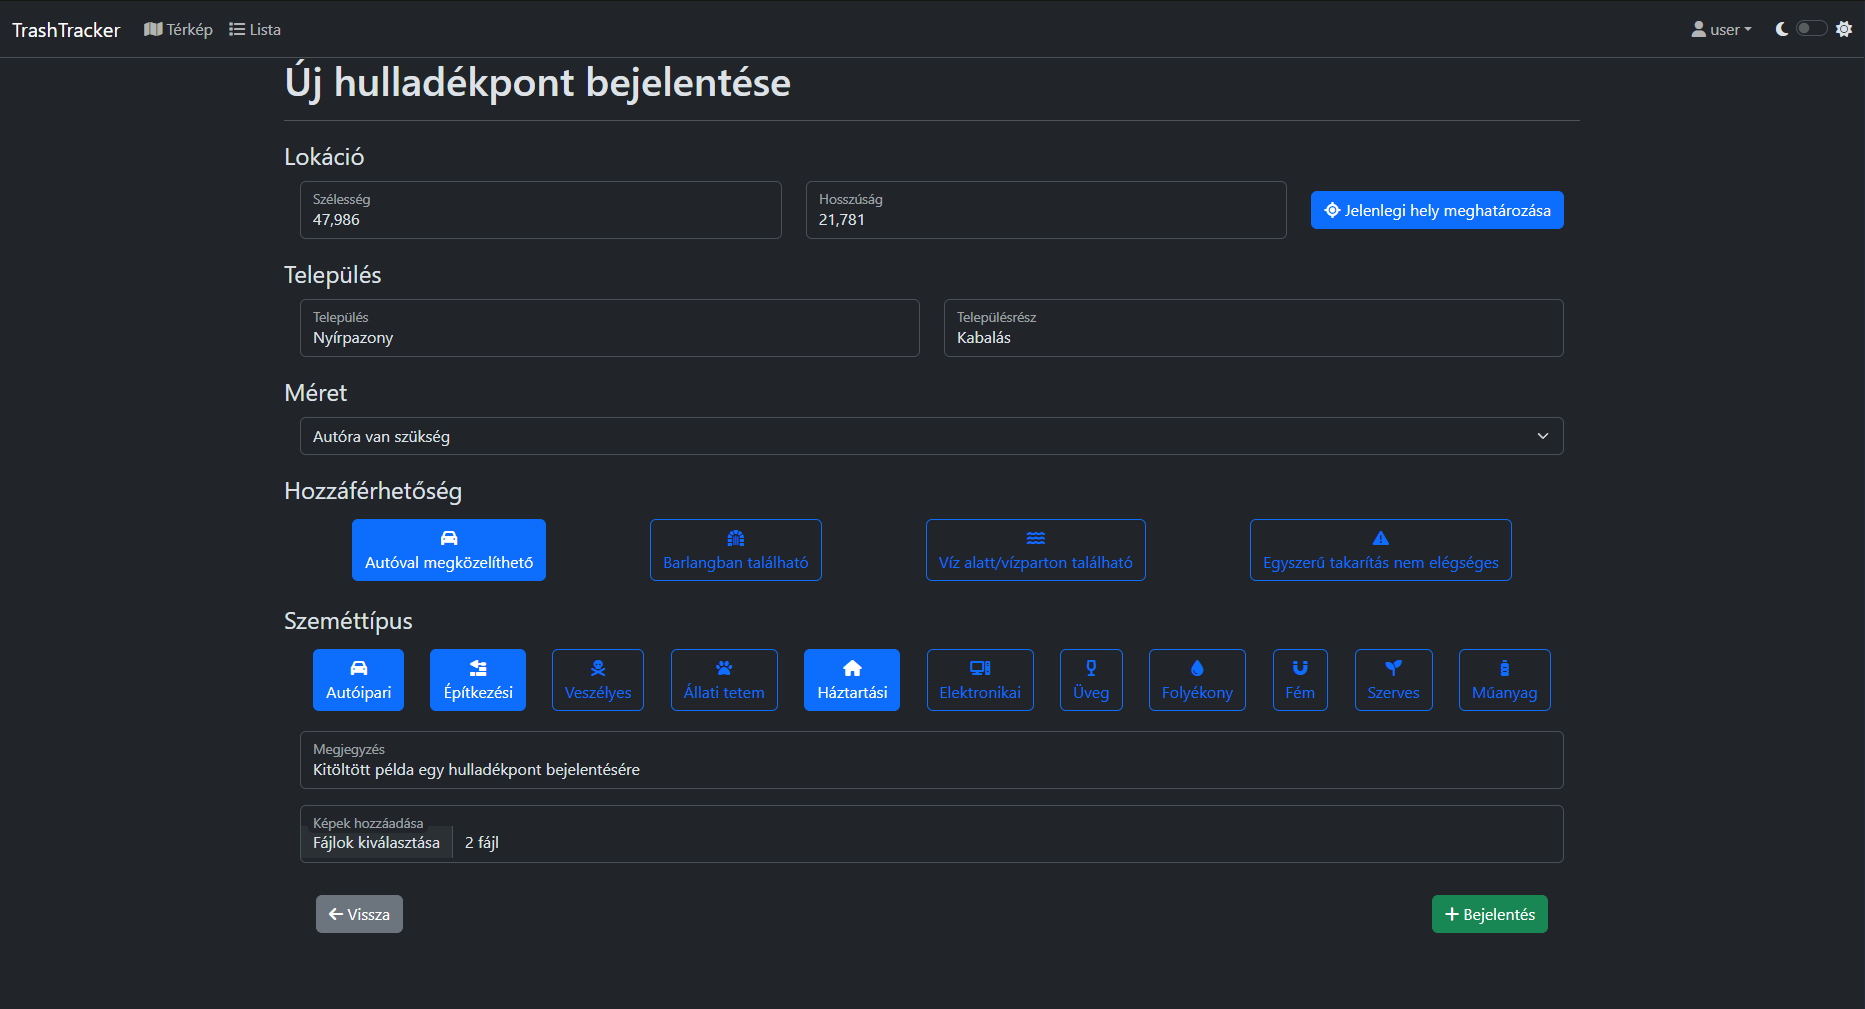
\includegraphics[width=0.7\textwidth]{trash_create}
	\caption{Szemétpont bejelentésének űrlapja}
	\label{fig:trash_create}
\end{figure}

\subsubsection{Hibaüzenetek}
\label{subsubsec:trash_create_errors}

Egy pont bejelentésekor egyedül a koordináták megadása kötelező, de erősen ajánlott további adatok leírása, illetve fénykép csatolása is. Ha a felhasználó nem ad meg egy kötelező adatot vagy beküldés előtt törli azt, akkor az űrlap egy "\textit{<adat> megadása kötelező!}" hibaüzenettel jelzi azt az adott mező alatt. A koordinátákkal kapcsolatosan vannak triviális követelmények is, mely szerint nem lehet kevesebb, mint -180 és több, mint 180, mely megsértésekor egy "\textit{A koordináta nem lehet kevesebb, mint -180° és több, mint 180°.}". Emellett az elfogadott formátum a tizedesvessző (tehát nem a -pont) használata. A megjegyzésbe bármit lehet írni, viszont biztonsági okokból az nem lehet több, mint 2000 karakter, mely túllépése esetén egy "\textit{2000 karakternél nem lehet hosszabb a megjegyzés!}". A képekkel kapcsolatosan van a legtöbb technikai követelmény, melyek kizárólag fájlok, azon belül is kép, ahol csak ".jpg" (vagy ".jpeg"), illetve ".png" formátumúak lehetnek, amelyek nem léphetik túl az 1 MB méretet. Ezen pontok megsértésekor rendre "\textit{Az objektum nem fájl!}", \textit{A fájl nem egy kép!}", "\textit{Ez a kép formátuma nem támogatott! Támogatott formátumok: ".jpg", ".jpeg", ".png".}", illetve "\textit{Ez a kép túl nagy! Maximális méret: 1024KB.}" hibaüzenetekkel találkozhat a felhasználó. \textbf{A bejelentés csak akkor véglegesedik, ha hiba nélkül sikerül megadni az adatokat!}

\subsection{Pont módosítása}
\label{subsec:trash_edit}

Egy már meglévő pont adatainak módosítására az azt részletező adatlap alján található "Módosítás", vagy a listanézet egyes soraiban található \faIcon{edit} ikonra kattintva érhető el. Az ezen az oldalon található űrlap hasonló, a pont létrehozáskor használtéhoz, a szemét állapotának lenyíló menüjét leszámítva, melynek megadása létrehozáskor még értelmetlen lenne. Emellett a meglevő képek felülírása helyett az itt megadottak (a hozzátartozó mező leírásához hűen) a ponthoz hozzáadásra kerülnek, a régieket megtartva.

\begin{figure}[H]
	\centering
	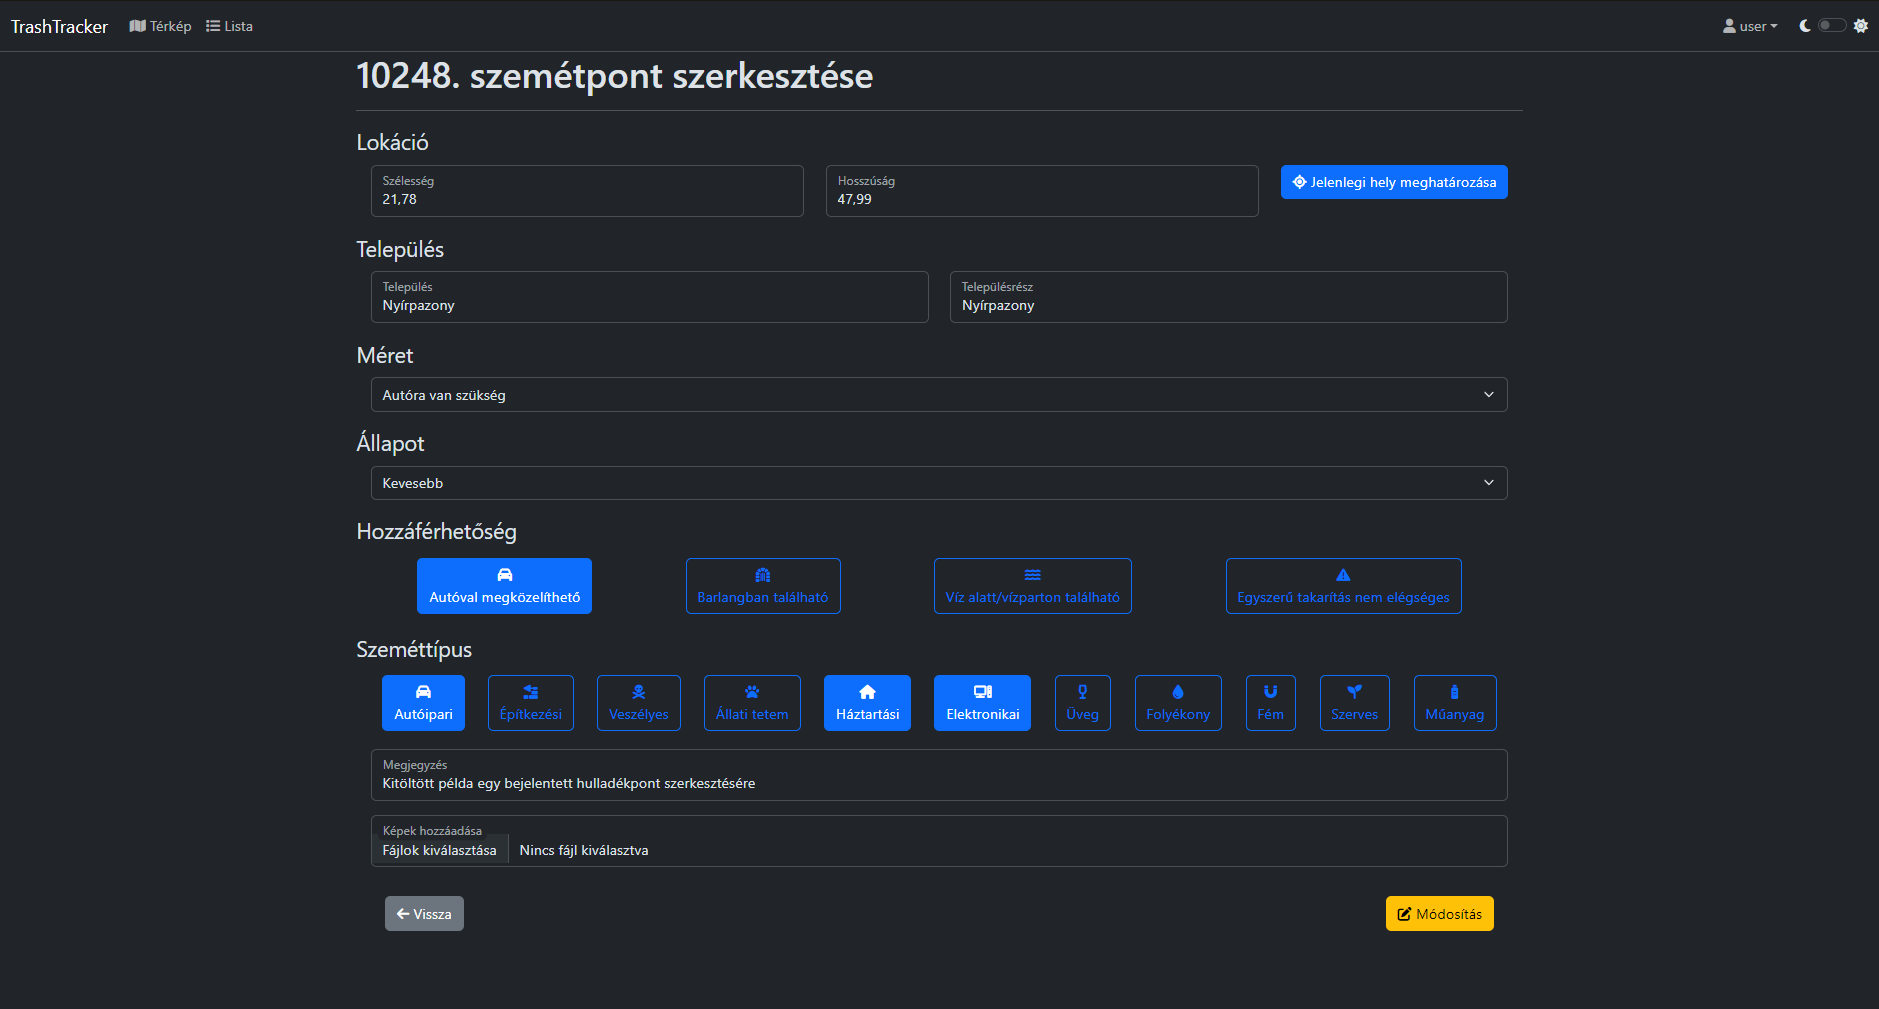
\includegraphics[width=0.7\textwidth]{trash_edit}
	\caption{Szemétpont módosításának űrlapja}
	\label{fig:trash_edit}
\end{figure}

\subsubsection{Hibaüzenetek}

Az itt megjelenő hibaüzenetek azonosak a \ref{subsubsec:trash_create_errors} bekezdésben tárgyaltakkal.

\subsection{Saját profil megtekintése}
\label{subsec:user_details}

A felhasználó regisztrálásával mindenki egy saját profil oldalra is szert tesz. A saját megtekintéséhez a navigációs sáv jobb oldalán, a felhasználónévre kattintva lenyíló menüben a "Saját profil" menüpontra nyomva van lehetőség.\\
Minden profiloldal fejlécében a bal oldalon a profilkép (ha van, ellenben egy "\textit{Nincs profilkép}" felirat), mellette pedig a felhasználó neve, illetve elérhetősége (e-mail címe) található. Ha a saját profilunk böngésszük, akkor az elérhetőségünk mellett találjuk a "Profil szerkesztése" gombot, mely értelemszerűen annak a szerkesztését segítő űrlapra navigál. Ez alatt az adott felhasználó által bejelentett pontok listanézete található, amely használata azonos a \ref{subsec:trash_index} bekezdésben tárgyaltakkal, a szűrési lehetőségeket leszámítva.

\begin{figure}[H]
	\centering
	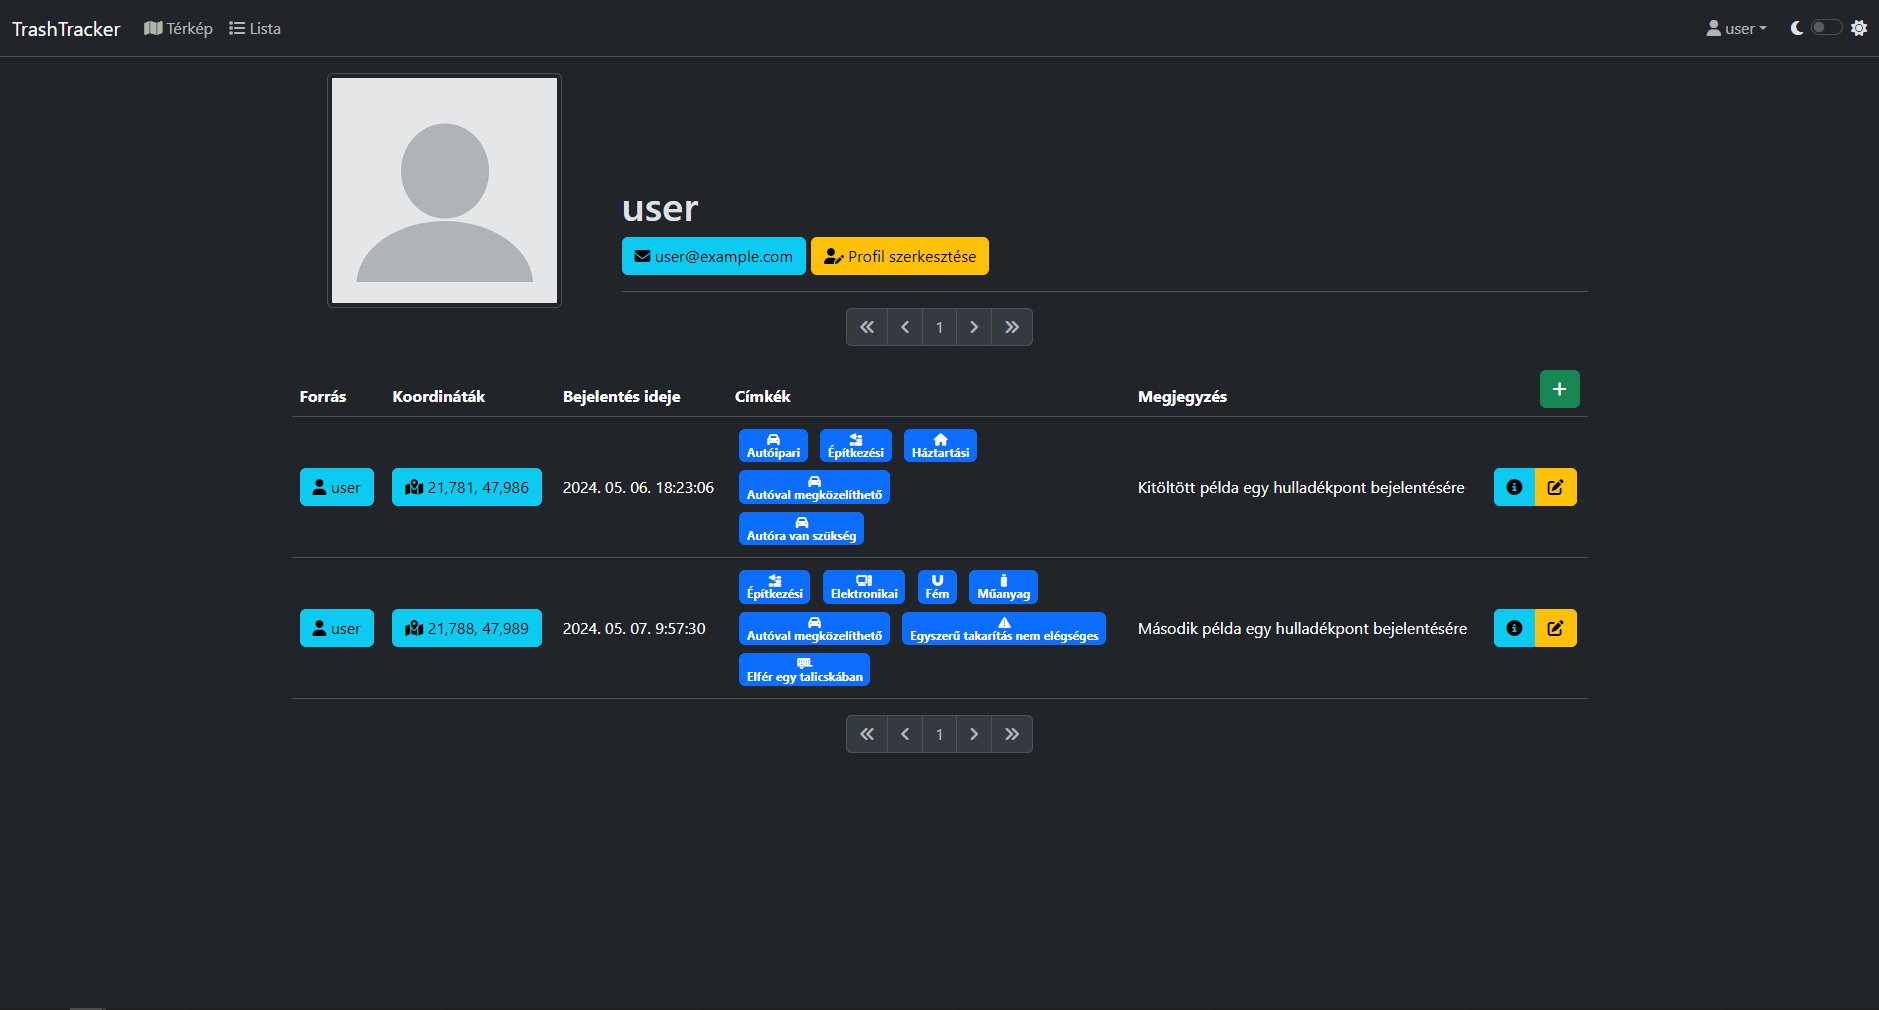
\includegraphics[width=0.7\textwidth]{user_details}
	\caption{Példa egy felhasználói profilra}
	\label{fig:user_details}
\end{figure}

\subsubsection{Más felhasználó profiljának megtekintése}

Egyszerű felhasználói fiókkal nincs lehetőség további felhasználók "felderítésére", csak az általuk bejelentett pontokon levő hivatkozásokkal. Mind a pontok listanézetében (\ref{subsec:trash_index} bekezdés), illetve azok adatlapján (\ref{subsec:trash_details} bekezdés) találhatóak ezek, ahol az adott fejezetekben tárgyaltak szerinti \faIcon{user} ikonnal ellátott gombokra kattintva van lehetőség.

\subsection{Saját profil szerkesztése}
\label{subsec:user_edit}

A saját profil megtekintésekor (\ref{subsec:user_details} bekezdés) a "Profil szerkesztése" gombra kattintva van lehetőség a felhasználónév, e-mail cím és profilkép módosítására. Ehhez is egy űrlap áll a rendelkezésre, mely a gombra kattintáskor jelenik meg, az előbb említett adatok mezőivel. Az alján található "Módosítás"-ra nyomva azok a mezők, melyek tartalmaznak adatot, és ha tartalmaznak akkor újat, módosulni fognak, feltéve ha hiba nélkül megy végbe az.

\begin{figure}[H]
	\centering
	\subcaptionbox{Profil szerkesztésének űrlapja}{
		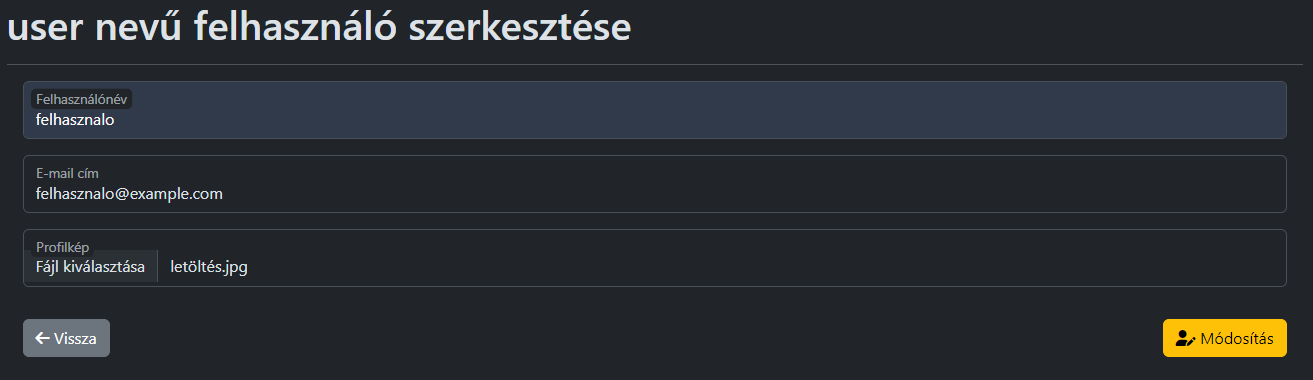
\includegraphics[width=0.4\textwidth]{user_edit}}
	\hspace{5pt}
	\subcaptionbox{Szerkesztés utáni profiloldal}{
		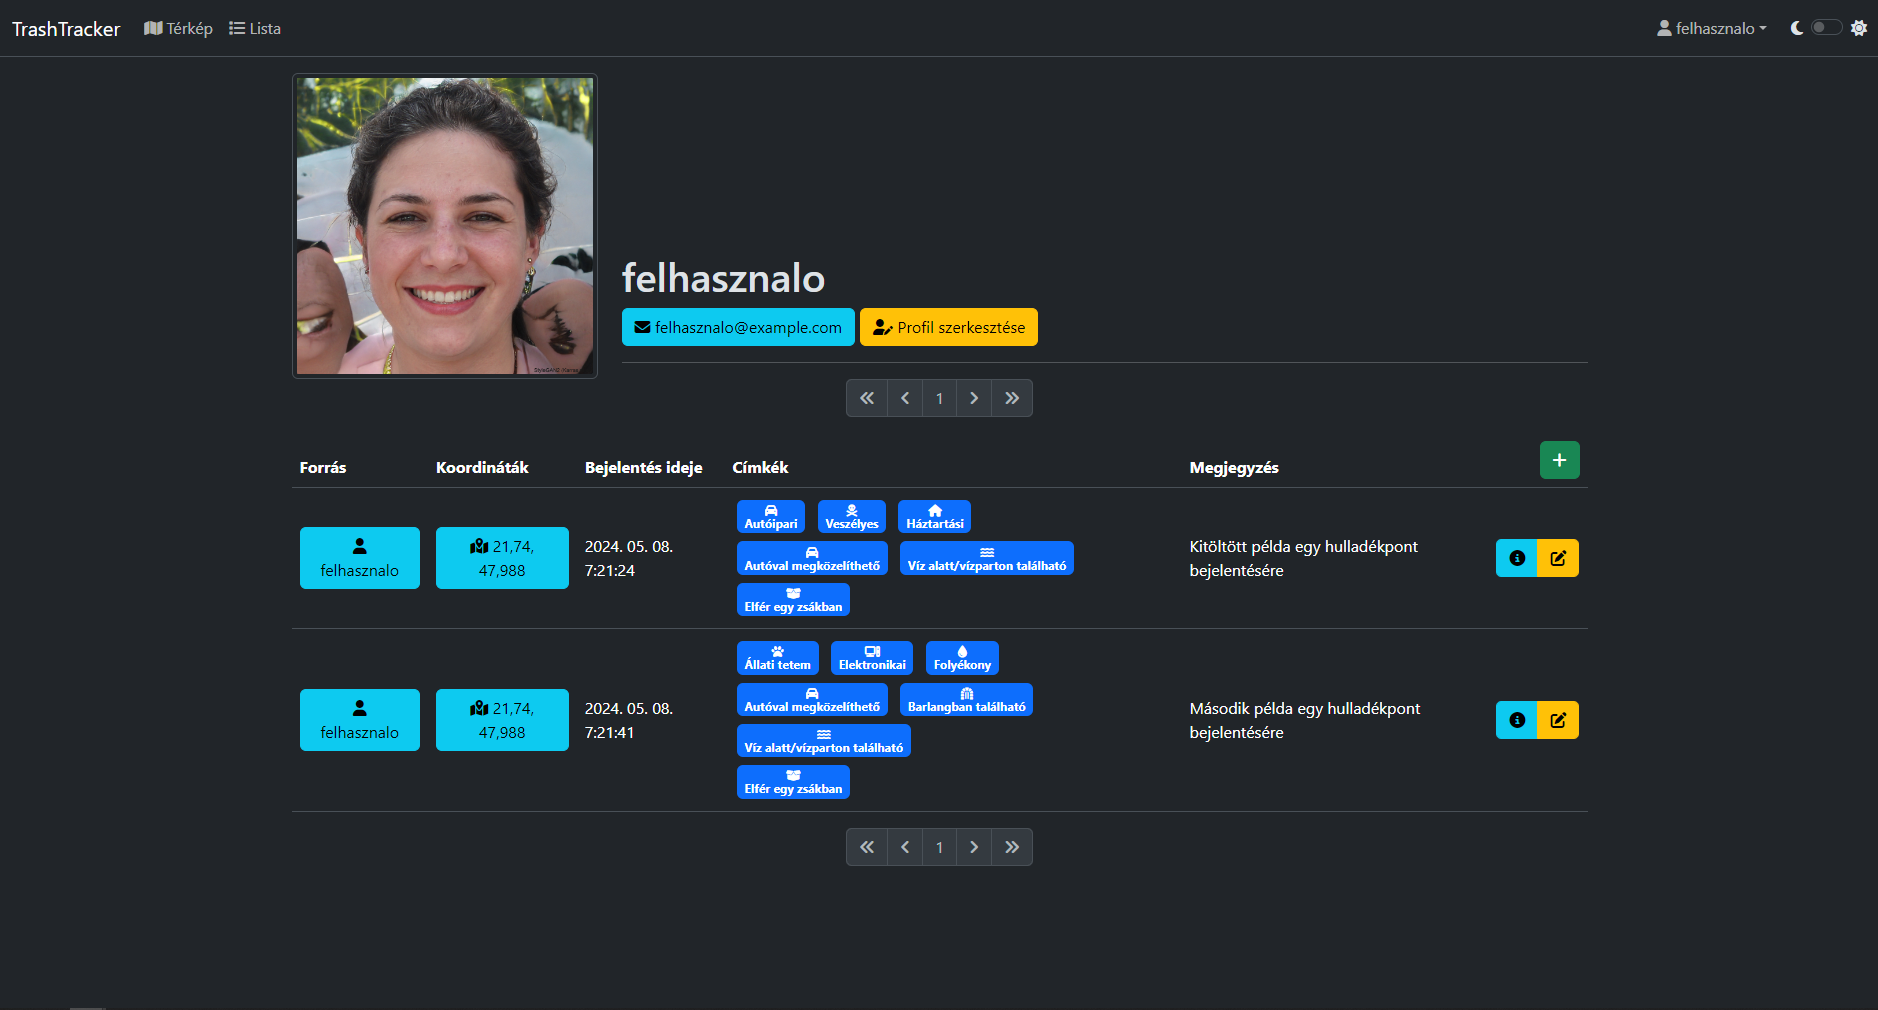
\includegraphics[width=0.55\linewidth]{user_details_edited}}
	\caption{Profil szerkesztése és annak eredménye}
	\label{fig:user_edit}
\end{figure}

\subsubsection{Hibaüzenetek}

Az űrlap elküldésekor van lehetőség, hogy sikeres módosítás helyett hibaüzenetet kapunk (ilyenkor az adatok nem módosulnak  még). Mivel minden felhasználónévnek és e-mail címnek egyedinek kell lennie, így ha azok mégsem lennének a módosítás után, 
akkor rendre "\textit{A felhasználónév már foglalt!}", illetve "\textit{Az e-mail cím már foglalt!}" üzenetekkel találkozhat a felhasználó. Emellett ez e-mail címnek érvényes formátumúnak kell lennie, és a profilképnek is meg kell felelnie a regisztráláskor definiáltakkal, mely a \ref{subsubsec:user_register_errors} bekezdésben van tárgyalva.

\begin{figure}[H]
	\centering
	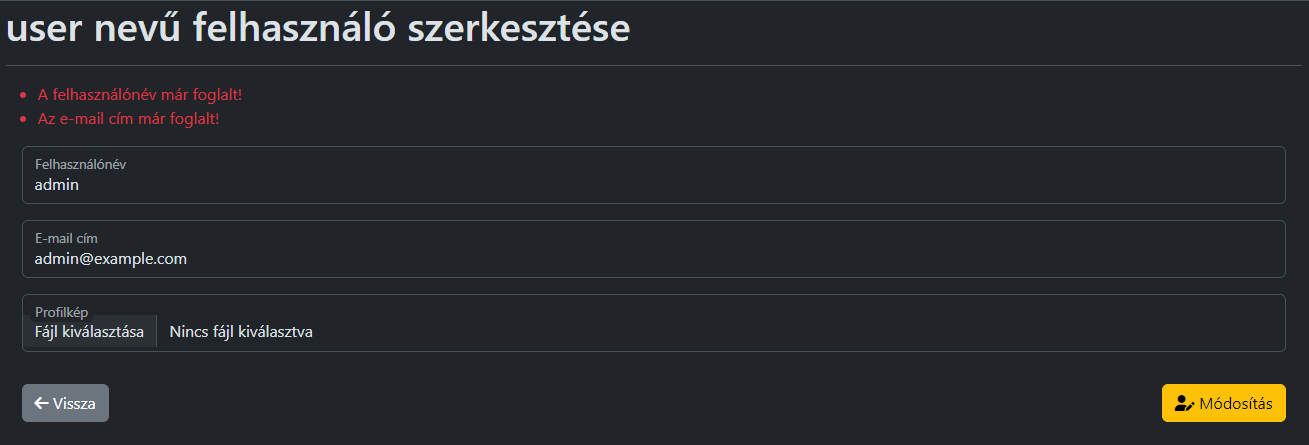
\includegraphics[width=0.7\textwidth]{user_edit_errors}
	\caption{Profil szerkesztésének űrlapja}
	\label{fig:user_edit_errors}
\end{figure}

\subsection{Kijelentkezés}
\label{subsec:logout}

Egy felhasználói fiókba való bejelentkezést követően természetesen lehetőség van az abból való kijelentkezésre is. A bejelentkezés státusza minden oldal navigációs sávján, annak jobb szélén található. A bejelentkezett fiók nevére kattintva lenyílik egy, a bejelentkezés/regisztrációnál megismert almenü, melyben a saját profil megtekintése mellett itt van lehetőség kijelentkezni, a "Kijelentkezés" pontra kattintva. Ekkor a felhasználó a főoldalra lesz navigálva, illetve újra vendégnek fog számítani, egy újabb bejelentkezésig.

\begin{figure}[H]
	\centering
	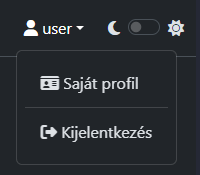
\includegraphics[width=0.25\textwidth]{logout}
	\caption{Bejelentkezett állapotban megváltozó almenü}
	\label{fig:logout}
\end{figure}


\section{Funkciók moderátorként}

A moderátor szintű felhasználói fiókok mindenre jogosultak, mint az egyszerű felhasználók, viszont képesek bejelentett pontok törlésére, ezzel az esetleges "spam" moderálására.

\begin{figure}[H]
	\centering
	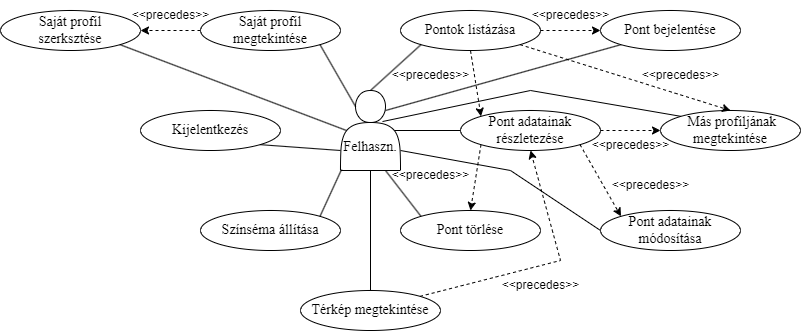
\includegraphics[width=1.0\textwidth]{usecase_moderator}
	\caption{Felhasználói esetek moderátorként}
	\label{fig:usecase_moderator}
\end{figure}

\subsection{Pont törlése}
\label{subsec:trash_delete}

Egy pont törlésére azok listanézetéből a \faIcon{trash} ikonra vagy annak adatlapján található "Törlés" gombra kattintva van lehetőség. A "balesetek" elkerülése érdekében először egy megerősítő oldalra navigál, ahol "Vissza" és "Törlés" opciók közül lehet választani, melyek rendre az előző oldalra navigálnak (törlés nélkül), illetve véglegesen törlik az adott pontot.

\begin{figure}[H]
	\centering
	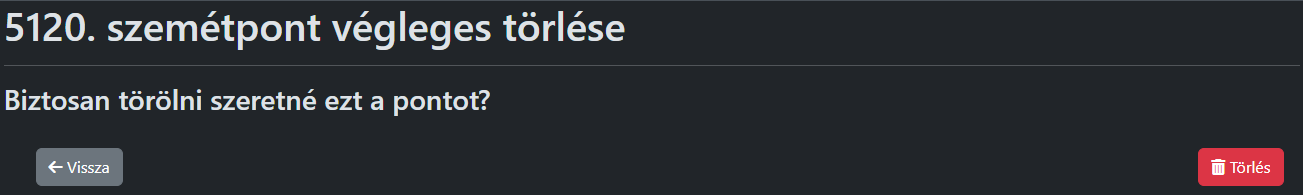
\includegraphics[width=0.7\textwidth]{trash_delete}
	\caption{Pont törlésének megerősítő űrlapja}
	\label{fig:trash_delete}
\end{figure}

\section{Funkciók adminisztrátorként}

Az adminisztrátori szintű fiókok mindenre jogosultak, tehát az előbb említett funkciók mellett képes a felhasználói fiókok listázására, azok módosítására, illetve törlésére is.

\begin{figure}[H]
	\centering
	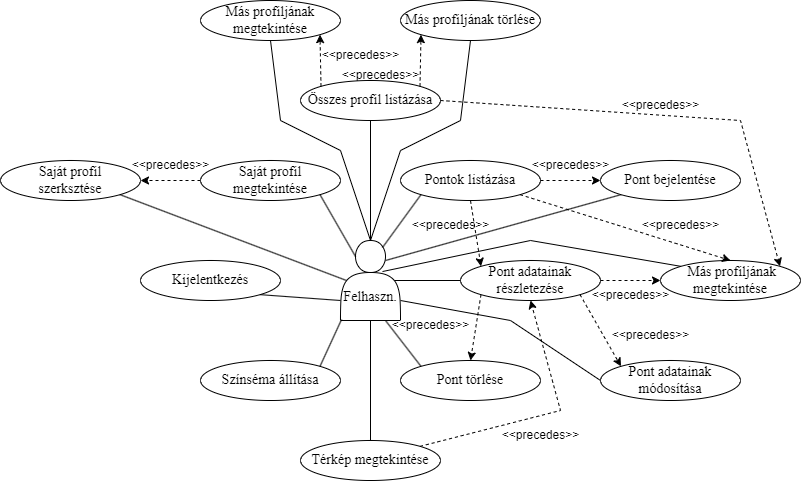
\includegraphics[width=1.0\textwidth]{usecase_admin}
	\caption{Felhasználói esetek adminisztrátorként}
	\label{fig:usecase_admin}
\end{figure}

\subsection{Felület áttekintése}
\label{subsec:nav_admin}

A \ref{subsec:nav_guest} bekezdésben tárgyalt navigációs felületen adminisztrátorként egy újabb hivatkozás válik elérhetővé "Felhasználók" névvel. Erre való kattintással elérhető az összes felhasználói fiók listázása.

\subsection{Felhasználói fiókok listázása}
\label{subsec:user_index}

Ez a felület a \ref{subsec:nav_admin} bekezdésben tárgyalt navigációs sávban található menüponttal érhető el, ha adminisztrátori szintű fiókkal van a felhasználó bejelentkezve. Kezelése hasonló a \ref{subsec:trash_index} bekezdésben tárgyalt szemétpontok listanézetével. A lista tetején ugyanúgy megtalálható a már megismert szűrő beállítások, ahol felhasználó vagy e-mail cím alapján lehet keresni, illetve a találatok lapszámát állítani. Ez alatt található a lista, ahol minden fiók felhasználónevét, e-mail címét és regisztrálási idejét (ha alapértelmezetten generált fiók, akkor az érték "0001. 01. 01. 0:00:00") lehet megtalálni, regisztrálás ideje szerint sorrendben (azaz a legfrissebb fiókok vannak előbb). Emellett minden rekord végén található három gomb, mely rendre az adott fiókhoz tartozó profil megtekintésére, -szerkesztésére és törlésére szolgál.

\begin{figure}[H]
	\centering
	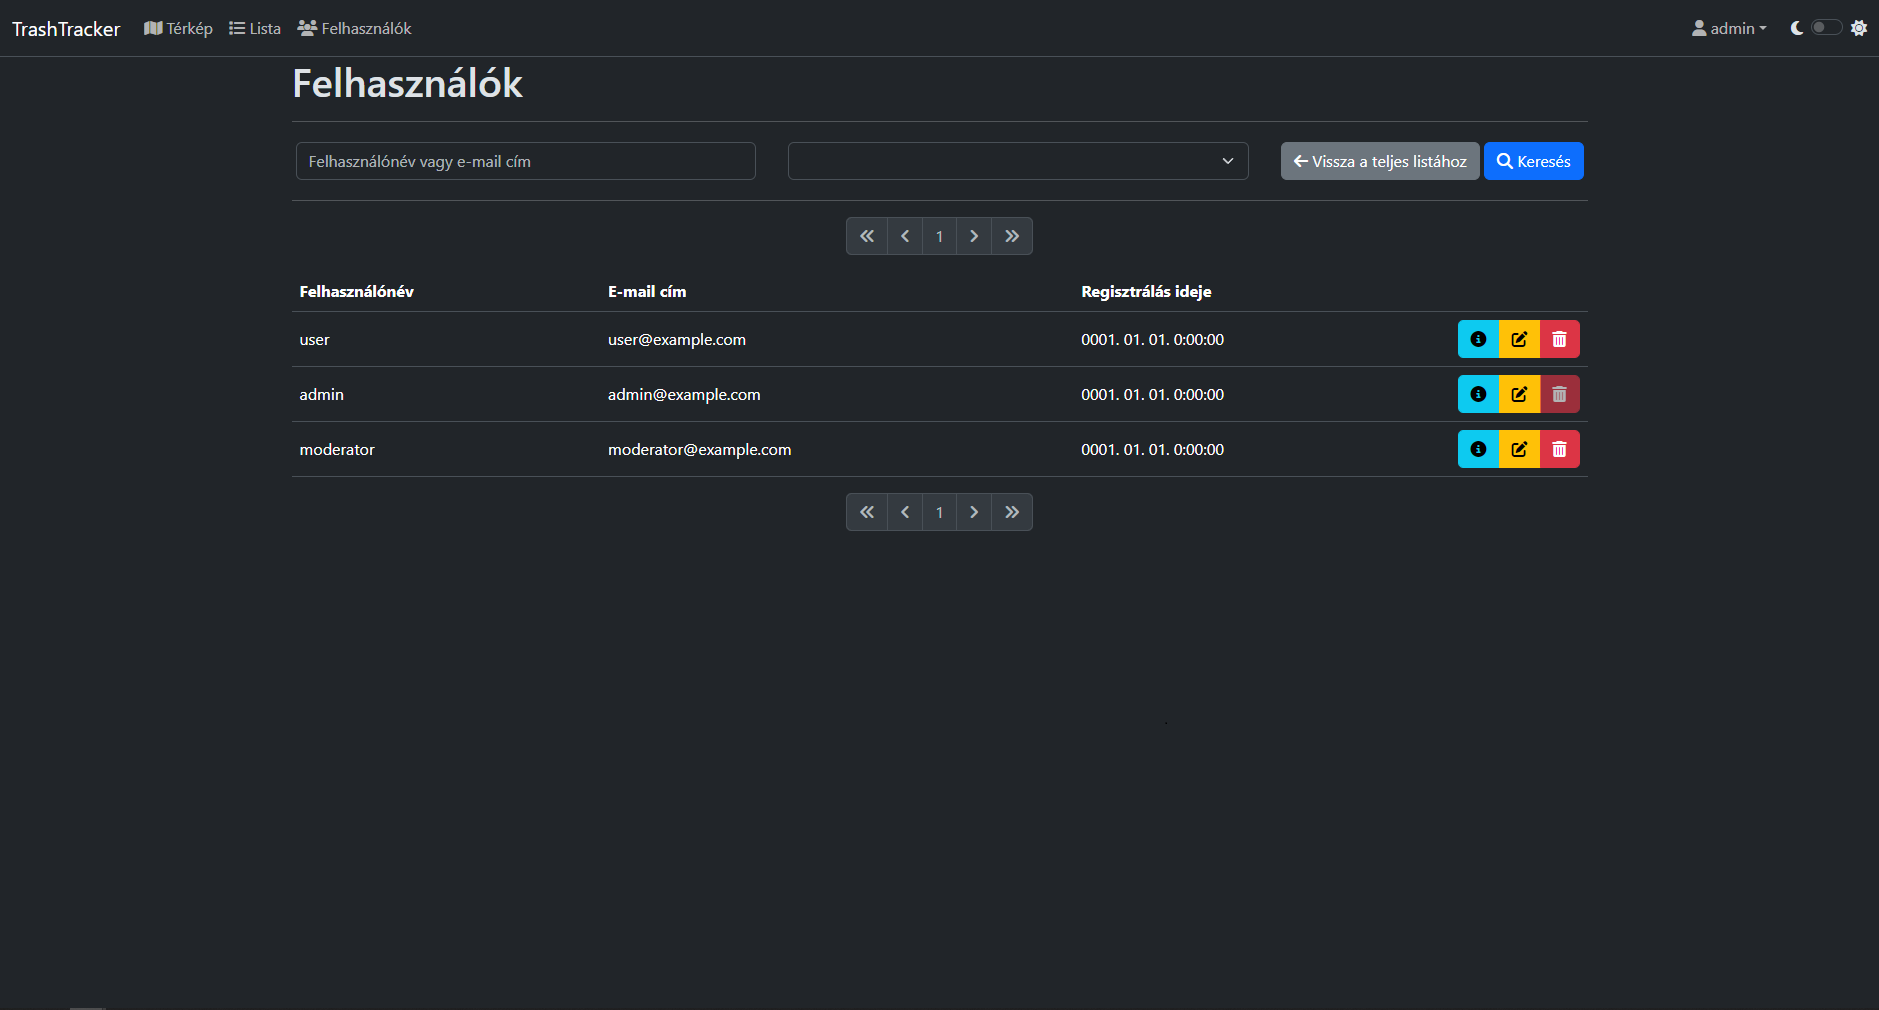
\includegraphics[width=0.7\textwidth]{user_index}
	\caption{Felhasználói fiókok listanézetének felülete}
	\label{fig:user_index}
\end{figure}

\subsection{Felhasználói fiókok módosítása}
\label{subsec:user_edit_admin}

A módosítás űrlapja hasonló, a \ref{subsec:user_edit} bekezdésben tárgyaltakkal, viszont itt lehetőség van egy adott felhasználói fiók hozzáférési szintjét állítani egy lenyíló lista segítségével. Biztonsági okok miatt a saját felhasználó jogosultsági köre nem módosítható, az erre való lista nem jelenik meg az űrlapon.

\begin{figure}[H]
	\centering
	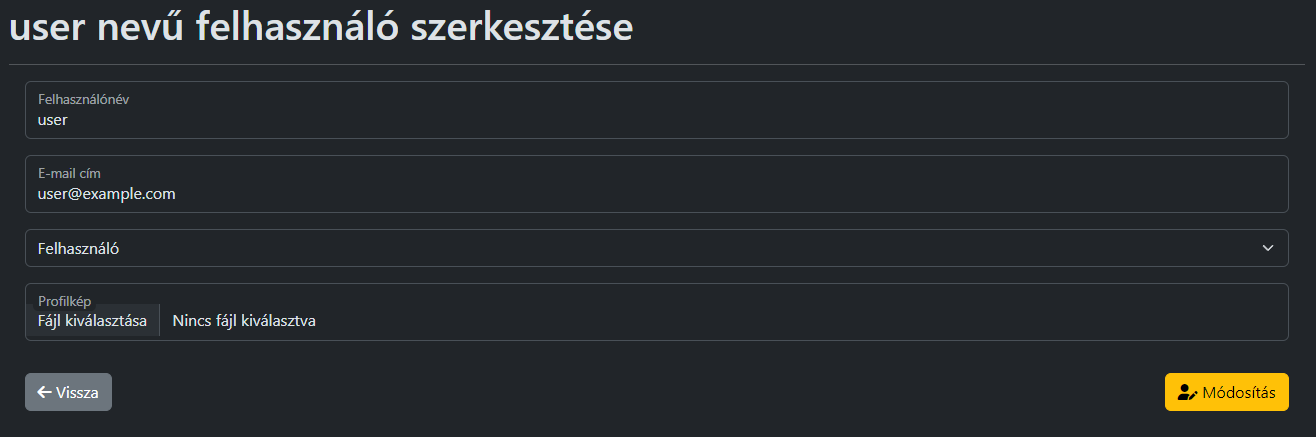
\includegraphics[width=0.7\textwidth]{user_edit_admin}
	\caption{Felhasználói fiókok szerkesztési űrlapja adminisztrátorként}
	\label{fig:user_edit_admin}
\end{figure}

\subsection{Felhasználói fiókok törlése}
\label{subsec:user_delete}

A törlés folyamata is megegyezik a \ref{subsec:trash_delete} bekezdésben tárgyalt pontéval. Biztonsági okok miatt, a saját felhasználót törölni nem lehet, a listában is az erre mutató gombhivatkozás nem kattintható.

\begin{figure}[H]
	\centering
	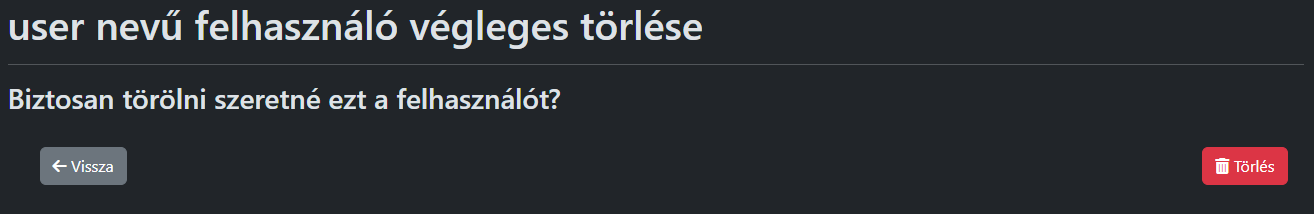
\includegraphics[width=0.7\textwidth]{user_delete}
	\caption{Felhasználói fiókok törlésének megerősítő űrlapja}
	\label{fig:user_delete}
\end{figure}
\cleardoublepage

\chapter{Fejlesztői dokumentáció}
\label{ch:impl}

Lorem ipsum dolor sit amet, consectetur adipiscing elit. Duis nibh leo, dapibus in elementum nec, aliquet id sem. Suspendisse potenti. Nullam sit amet consectetur nibh. Donec scelerisque varius turpis at tincidunt.


\section{Tételek, definíciók, megjegyzések}

\begin{definition}
Mauris tristique sollicitudin ultrices. Etiam tristique quam sit amet metus dictum imperdiet. Nunc id lorem sed nisl pulvinar aliquet vitae quis arcu. Morbi iaculis eleifend porttitor.
\end{definition}

Maecenas rutrum eros sem, pharetra interdum nulla porttitor sit amet. In vitae viverra ante. Maecenas sit amet placerat orci, sed tincidunt velit. Vivamus mattis, enim vel suscipit elementum, quam odio venenatis elit, et mollis nulla nunc a risus. Praesent purus magna, tristique sed lacus sit amet, convallis malesuada magna. Phasellus faucibus varius purus, nec tristique enim porta vitae.

\begin{theorem}
Nulla finibus ante vel arcu tincidunt, ut consectetur ligula finibus. Mauris mollis lectus sed ipsum bibendum, ac ultrices erat dictum. Suspendisse faucibus euismod lacinia. Etiam vel odio ante.
\end{theorem}
\begin{proof}
Etiam pulvinar nibh quis massa auctor congue. Pellentesque quis odio vitae sapien molestie vestibulum sit amet et quam. Pellentesque vel dui eget enim hendrerit finibus at sit amet libero. Quisque sollicitudin ultrices enim, nec porta magna imperdiet vitae. Cras condimentum nunc dui.
\end{proof}

Donec dapibus sodales ante, at scelerisque nunc laoreet sit amet. Mauris porttitor tincidunt neque, vel ullamcorper neque pulvinar et. Integer eu lorem euismod, faucibus lectus sed, accumsan felis. 

\begin{remark}
Nunc ornare mi at augue vulputate, eu venenatis magna mollis. Nunc sed posuere dui, et varius nulla. Sed mollis nibh augue, eget scelerisque eros ornare nec. Praesent porta, metus eget eleifend consequat, eros ligula eleifend ex, a pellentesque mi est vitae urna. Vivamus turpis nunc, iaculis non leo eget, mattis vulputate tellus.
\end{remark}

Fusce in aliquet neque, in pretium sem. Donec tincidunt tellus id lectus pretium fringilla. Nunc faucibus, erat pretium tempus tempor, tortor mi fringilla neque, ac congue ex dui vitae mauris. Donec pretium et quam a cursus.

\begin{note}
Aliquam vehicula luctus mi a pretium. Nulla quam neque, maximus nec velit in, aliquam mollis tortor. Aliquam erat volutpat. Curabitur vitae laoreet turpis. Integer id diam ligula.
\end{note}

Ut sollicitudin tempus urna et mollis. Aliquam et aliquam turpis, sed fermentum mauris. Nulla eget ex diam. Donec eget tellus pharetra, semper neque eget, rutrum diam.

\subsection{Egyenletek, matematika}

Duis suscipit ipsum nec urna blandit, $2 + 2 = 4$ pellentesque vehicula quam fringilla. Vivamus euismod, lectus sit amet euismod viverra, dolor metus consequat sapien, ut hendrerit nisl nulla id nisi. Nam in leo eu quam sollicitudin semper a quis velit.

$$a^2 + b^2 = c^2$$

Phasellus mollis, elit sed convallis feugiat, dolor quam dapibus nibh, suscipit consectetur lacus risus quis sem. Vivamus scelerisque porta odio, vitae euismod dolor accumsan ut.

In mathematica, identitatem Euleri (equation est scriptor vti etiam notum) sit aequalitatem \ref{eq:euler}.~egyenlet:
\begin{equation}\label{eq:euler}
e^{i \times \pi} + 1 = 0
\end{equation}

Vestibulum ante ipsum primis in faucibus orci luctus et ultrices posuere cubilia curae; Nullam pulvinar purus at pharetra elementum.
Aequationes adsignans aequationis signum:
\begin{align}
	A & = \frac{\pi r^2}{2} \\
	  & = \frac{1}{2} \pi r^2
\end{align}

Proin tempor risus a efficitur condimentum. Cras lobortis ligula non sollicitudin euismod. Fusce non pellentesque nibh, non elementum tellus.
Omissa numeratione aliquarum aequationum:
\begin{align}
	f(u) & =\sum_{j=1}^{n} x_jf(u_j) \nonumber \\
	     & =\sum_{j=1}^{n} x_j \sum_{i=1}^{m} a_{ij}v_i \nonumber \\
	     & =\sum_{j=1}^{n} \sum_{i=1}^{m} a_{ij}x_jv_i
\end{align}

\section{Forráskódok}

Nulla sodales purus id mi consequat, eu venenatis odio pharetra. Cras a arcu quam. Suspendisse augue risus, pulvinar a turpis et, commodo aliquet turpis. Nulla aliquam scelerisque mi eget pharetra. Mauris sed posuere elit, ac lobortis metus. Proin lacinia sit amet diam sed auctor. Nam viverra orci id sapien sollicitudin, a aliquam lacus suscipit. Quisque ac tincidunt leo \ref{src:cpp}. és \ref{src:csharp}.~forráskód:

\lstset{caption={Hello World in C++}, label=src:cpp}
\begin{lstlisting}[language={C++}]
#include <stdio>

int main() 
{
	int c;
	std::cout << "Hello World!" << std::endl;

	std::cout << "Press any key to exit." << std::endl;
	std::cin >> c;
	
	return 0;
}
\end{lstlisting}

\lstset{caption={Hello World in C\#}, label=src:csharp}
\begin{lstlisting}[language={[Sharp]C}]
using System;
namespace HelloWorld
{
	class Hello 
	{
		static void Main() 
		{
			Console.WriteLine("Hello World!");
			
			Console.WriteLine("Press any key to exit.");
			Console.ReadKey();
		}
	}
}
\end{lstlisting}

\subsection{Algoritmusok}

Az \ref{alg:ibb}.~algoritmus egy általános elágazás és korlátozás algoritmust (\emph{Branch and Bound algorithm}) mutat be. A \ref{step:selrule}.~lépésben egy megfelelő kiválasztási szabályt kell alkalmazni.
Példa forrása: \href{https://www.inf.u-szeged.hu/actacybernetica/}{Acta Cybernetica (ez egy hiperlink)}.

\begin{algorithm}[H]
\caption{A general interval B\&B algorithm}
\label{alg:ibb}
\textbf{\underline{Funct}} IBB($S,f$)
\begin{algorithmic}[1] % sorszámok megjelenítése minden n. sor előtt, most n = 1
\State Set the working list ${\cal L}_W$ := $\{S\}$ and the final list ${\cal L}_Q$ := $\{\}$
\While{( ${\cal L}_W \neq \emptyset$ )} \label{alg:igoend}
	\State Select an interval $X$ from ${\cal L}_W$ \label{step:selrule}\Comment{Selection rule}
	\State Compute $lbf(X)$ \Comment{Bounding rule}
	\If{$X$ cannot be eliminated} \Comment{Elimination rule}
		\State Divide $X$ into $X^j,\ j=1,\dots, p$, subintervals   \Comment{Division rule}
		\For{$j=1,\ldots,p$}
			\If{$X^j$ satisfies the termination criterion} \Comment{Termination rule}
				\State Store $X^j$ in ${\cal L}_W$
			\Else
				\State Store $X^j$ in ${\cal L}_W$
			\EndIf
		\EndFor
	\EndIf
\EndWhile
\State \textbf{return} ${\cal L}_Q$
\end{algorithmic}
\end{algorithm}

\cleardoublepage

\chapter{Összegzés}
\label{ch:sum}

A leírtak szerint a környezetünkben található, nem megfelelően kezelt hulladék jelentős mértékben hozzájárul bolygónk egyre romló állapotához. Bár sok ember, akár teljes életpályáját ennek szentelve igyekszik ezen folyamatok megállításában, ennek ellenére ezek mégsem elegek. A legfőbb gond, hogy a legtöbb emberhez el sem jut, hogy mekkora hatása is van, akár csak ennek az egy jelenségnek, melyet a dolgozat során készült webalkalmazás is igyekszik orvosolni.\par
A dolgozattal implementált programmal jól látható, hogy a probléma a közösség erejével ha bár nem is teljesen felszámolható, de mindenképpen minimalizálható lehetne. A térképen vizualizált bejelentett illegális szemétlerakatok pontos helyzete már nagyban hozzájárul a környezetükért tenni akaró embereknek, akik akár szabadidejükben is tisztítják környezetüket azok után, akik ezt nem tisztelik.
\cleardoublepage

% Acknowledgements (optional) - in case your thesis received funding or would like to express special thanks to someone
\chapter*{\acklabel}
\addcontentsline{toc}{chapter}{\acklabel}
Amennyiben a szakdolgozati / diplomamunka projekted pénzügyi támogatást kapott egy projektből vagy az egyetemtől, jellemzően kötelező feltüntetni a dolgozatban is. A dolgozat elkészítéséhez segítséget nyújtó oktatók, hallgatótársak, kollégák felé is nyilvánítható külön köszönet.

% Appendices (optional) - useful for detailed information in long tables, many and/or large figures, etc.
\appendix
\chapter{Manuális teszteredmények}
\label{appx:simulation}

\section{Vendég}
\label{sec:sim_guest}

\begin{center}
	\centering
	\begin{longtable}{ | m{0.025\textwidth}| m{0.1\textwidth} | m{0.75\textwidth} | }
		\hline
		\multicolumn{3}{ | c | }{\textbf{Navigációs sáv} (\ref{subsec:nav_guest} alszakasz)} \\
		\hline
		\multicolumn{2}{ | l | }{AS A} & vendég \\
		\hline
		\multicolumn{2}{ | l | }{I WANT TO} & valamelyik aloldalra navigálni \\
		\hline
		\multicolumn{2}{ | l | }{SO THAT} & azt az aloldalt elérjem \\
		\hline
		\multirow{3}{*}{1} & GIVEN & bármely oldalon vagyok \\
		\cline{2-3}
		& WHEN & a navigációs sávban a "Térkép" feliratra kattintok \\
		\cline{2-3}
		& THEN & a főoldalra/térképre leszek navigálva \\
		\hline
		\multirow{3}{*}{2} & GIVEN & bármely oldalon vagyok \\
		\cline{2-3}
		& WHEN & a navigációs sávban a "Lista" feliratra kattintok \\
		\cline{2-3}
		& THEN & a pontok listanézetére leszek navigálva \\
		\hline
		\multirow{3}{*}{3} & GIVEN & bármely oldalon vagyok \\
		\cline{2-3}
		& WHEN & a navigációs sávban a "Nincs bejelentkezve" feliratra kattintok \\
		\cline{2-3}
		& THEN & lenyílik egy almenü, benne "Bejelentkezés" és "Regisztráció" feliratokkal \\
		\hline
		\multirow{3}{*}{4} & GIVEN & bármely oldalon vagyok, a "Nincs bejelentkezve" feliratra kattintva \\
		\cline{2-3}
		& WHEN & a lenyíló almenüben a "Bejelentkezés" feliratra kattintok \\
		\cline{2-3}
		& THEN & a bejelentkezési űrlapra leszek navigálva \\
		\hline
		\multirow{3}{*}{5} & GIVEN & bármely oldalon vagyok, a "Nincs bejelentkezve" feliratra kattintva \\
		\cline{2-3}
		& WHEN & a lenyíló almenüben a "Regisztráció" feliratra kattintok \\
		\cline{2-3}
		& THEN & a regisztrációs űrlapra leszek navigálva \\
		\hline
		\multirow{3}{*}{6} & GIVEN & bármely oldalon vagyok \\
		\cline{2-3}
		& WHEN & a jobb oldalon található színséma kapcsolóra kattintok \\
		\cline{2-3}
		& THEN & a weboldalak színsémája átvált sötét és világos között a másikba \\
		\hline
		\multirow{3}{*}{7} & GIVEN & bármely oldalon vagyok, nem az alapértelmezett (sötét) színsémával \\
		\cline{2-3}
		& WHEN & átnavigálok bármely aloldalra \\
		\cline{2-3}
		& THEN & a színséma megmarad az aloldalon is \\
		\hline
	\end{longtable}
	\label{tab:sim_guest_navigation}
\end{center}

\begin{center}
	\centering
	\begin{longtable}{ | m{0.025\textwidth}| m{0.1\textwidth} | m{0.75\textwidth} | }
		\hline
		\multicolumn{3}{ | c | }{\textbf{Térkép} (\ref{subsec:map_guest} alszakasz)} \\
		\hline
		\multicolumn{2}{ | l | }{AS A} & vendég (vagy felhasználó, moderátor, adminisztrátor) \\
		\hline
		\multicolumn{2}{ | l | }{I WANT TO} & térképen böngészni \\
		\hline
		\multicolumn{2}{ | l | }{SO THAT} & a térképet böngésszem \\
		\hline
		\multirow{3}{*}{1} & GIVEN & a főoldalon/térképen vagyok egy asztali számítógépen \\
		\cline{2-3}
		& WHEN & a térképre bal egérgombot húzva \\
		\cline{2-3}
		& THEN & a térképet mozgatom \\
		\hline
		\multirow{3}{*}{2} & GIVEN & a főoldalon/térképen vagyok egy asztali számítógépen \\
		\cline{2-3}
		& WHEN & a térképre egérgörgőt felfelé, illetve lefelé görgetve \\
		\cline{2-3}
		& THEN & a térképet nagyítom, illetve kicsinyítem \\
		\hline
		\multirow{3}{*}{3} & GIVEN & a főoldalon/térképen vagyok egy asztali számítógépen \\
		\cline{2-3}
		& WHEN & a térképre Shift billentyű nyomása mellett jobb egérgombot húzva \\
		\cline{2-3}
		& THEN & a térképet nagyítom/kicsinyítem és forgatom, az egérgomb lehúzásának kezdeti pozíciójához mérten \\
		\hline
		\multirow{3}{*}{4} & GIVEN & a főoldalon/térképen vagyok egy érintőképernyős eszközön \\
		\cline{2-3}
		& WHEN & a térképre nyomva ujjat húzva \\
		\cline{2-3}
		& THEN & a térképet mozgatom \\
		\hline
		\multirow{3}{*}{5} & GIVEN & a főoldalon/térképen vagyok egy érintőképernyős eszközön \\
		\cline{2-3}
		& WHEN & a térképre nyomva két ujjat széttolva, illetve összehúzva \\
		\cline{2-3}
		& THEN & a térképet nagyítom, illetve kicsinyítem \\
		\hline
		\multirow{3}{*}{6} & GIVEN & a főoldalon/térképen vagyok \\
		\cline{2-3}
		& WHEN & a térkép bal alsó sarkában található \faIcon{filter} gombra kattintva \\
		\cline{2-3}
		& THEN & a szűrési menü beúszik alulról \\
		\hline
		\multirow{3}{*}{7} & GIVEN & a főoldalon/térképen vagyok, a szűrési menüt megnyitva \\
		\cline{2-3}
		& WHEN & a menü bármely tulajdonságot ábrázoló gombjára kattintva \\
		\cline{2-3}
		& THEN & annak logikai állapota átvált és a térképen található pontok azoknak megfelelően szűrődnek \\
		\hline
		\multirow{3}{*}{8} & GIVEN & a főoldalon/térképen vagyok, a szűrési menüt megnyitva \\
		\cline{2-3}
		& WHEN & a menü jobb felső sarkában található $\times$ gombra kattintva \\
		\cline{2-3}
		& THEN & a szűrési menü bezárul \\
		\hline
		\multirow{3}{*}{9} & GIVEN & a főoldalon/térképen vagyok \\
		\cline{2-3}
		& WHEN & a térkép jobb alsó sarkában található \faIcon{download} gombra kattintva \\
		\cline{2-3}
		& THEN & a pontok .csv-be szedett formátumban fájlként letöltésre kerülnek \\
		\hline
		\multirow{3}{*}{10} & GIVEN & a főoldalon/térképen vagyok \\
		\cline{2-3}
		& WHEN & a térképen megjelenített pontra kattintva \\
		\cline{2-3}
		& THEN & a ponton egy modális buborékban megjelenik annak sorszáma, egy képe és megjegyzése, egy hivatkozással annak adatlapjára \\
		\hline
		\multirow{3}{*}{11} & GIVEN & a főoldalon/térképen vagyok, egy azon található pontra kattintva \\
		\cline{2-3}
		& WHEN & a modális buborékban található "Részletek" gombra kattintok \\
		\cline{2-3}
		& THEN & annak adatlapjára leszek navigálva \\
		\hline
		\multirow{3}{*}{12} & GIVEN & a főoldalon/térképen vagyok, egy azon található pontra kattintva \\
		\cline{2-3}
		& WHEN & a modális buborékra kétszer kattintok \\
		\cline{2-3}
		& THEN & a buborékot bezárom \\
		\hline
	\end{longtable}
	\label{tab:sim_guest_map}
\end{center}

\begin{center}
	\centering
	\begin{longtable}{ | m{0.025\textwidth}| m{0.1\textwidth} | m{0.75\textwidth} | }
		\hline
		\multicolumn{3}{ | c | }{\textbf{Pont részletezése (\ref{subsec:trash_details} alszakasz)}} \\
		\hline
		\multicolumn{2}{ | l | }{AS A} & vendég \\
		\hline
		\multicolumn{2}{ | l | }{I WANT TO} & pont adatlapját megtekinteni \\
		\hline
		\multicolumn{2}{ | l | }{SO THAT} & a pont adatlapján szereplő adatokat megismerni \\
		\hline
		\multirow{3}{*}{1} & GIVEN & a pont adatlapján vagyok \\
		\cline{2-3}
		& WHEN & a pont feltöltőjére vagy forrására kattintok \\
		\cline{2-3}
		& THEN & a pont feltöltőjének profiljára vagy annak forrására leszek navigálva \\
		\hline
		\multirow{3}{*}{2} & GIVEN & a pont adatlapján vagyok \\
		\cline{2-3}
		& WHEN & a pont koordinátáira kattintok \\
		\cline{2-3}
		& THEN & a térképre leszek navigálva, az adott pontra nagyítva \\
		\hline
	\end{longtable}
	\label{tab:sim_guest_trash_details}
\end{center}

\begin{center}
	\centering
	\begin{longtable}{ | m{0.025\textwidth}| m{0.1\textwidth} | m{0.75\textwidth} | }
		\hline
		\multicolumn{3}{ | c | }{\textbf{Pontok listanézete (\ref{subsec:trash_index} alszakasz)}} \\
		\hline
		\multicolumn{2}{ | l | }{AS A} & vendég \\
		\hline
		\multicolumn{2}{ | l | }{I WANT TO} & pontok listanézetét megtekinteni \\
		\hline
		\multicolumn{2}{ | l | }{SO THAT} & a pontok listanézetben böngésszem \\
		\hline
		\multirow{3}{*}{1} & GIVEN & a pont listanézetének oldalán vagyok \\
		\cline{2-3}
		& WHEN & a szűrési feltételeket megadva a "Keresés" gombra kattintok \\
		\cline{2-3}
		& THEN & a listát az azoknak megfelelő pontokkal az ott megadott oldalméretben kapom vissza \\
		\hline
		\multirow{3}{*}{2} & GIVEN & a pont listanézetének oldalán vagyok \\
		\cline{2-3}
		& WHEN & a "Vissza a teljes listához" gombra kattintok \\
		\cline{2-3}
		& THEN & a listát alapértelmezett (100 pont/oldal, meg nem tisztított összes pont) keresési feltételeivel kapom vissza \\
		\hline
		\multirow{3}{*}{3} & GIVEN & a pont listanézetének oldalán vagyok \\
		\cline{2-3}
		& WHEN & egy oldalszámra vagy a \faIcon{angle-double-left}, \faIcon{angle-left}, \faIcon{angle-right}, \faIcon{angle-double-right} ikonok valamelyikére kattintok \\
		\cline{2-3} 
		& THEN & az adott számú, vagy az első, előző, következő, illetve utolsó oldalra leszek navigálva \\
		\hline
		\multirow{3}{*}{4} & GIVEN & a pont listanézetének oldalán vagyok \\
		\cline{2-3}
		& WHEN & az egyik pont (sor) feltöltőjére vagy forrására kattintok \\
		\cline{2-3}
		& THEN & az adott pont feltöltőjének profiljára vagy forrására leszek navigálva \\
		\hline
		\multirow{3}{*}{5} & GIVEN & a pont listanézetének oldalán vagyok \\
		\cline{2-3}
		& WHEN & az egyik pont (sor) koordinátáira kattintok \\
		\cline{2-3}
		& THEN & a térképre leszek navigálva, az adott pontra nagyítva \\
		\hline
		\multirow{3}{*}{6} & GIVEN & a pont listanézetének oldalán vagyok \\
		\cline{2-3}
		& WHEN & az egyik pont (sor) jobb végén található \faIcon{info-circle} gombra kattintok \\
		\cline{2-3}
		& THEN & annak adatlapjára leszek navigálva \\
		\hline
	\end{longtable}
	\label{tab:sim_guest_trash_index}
\end{center}

\begin{center}
	\centering
	\begin{longtable}{ | m{0.025\textwidth}| m{0.1\textwidth} | m{0.75\textwidth} | }
		\hline
		\multicolumn{3}{ | c | }{\textbf{Regisztráció (\ref{subsec:register} alszakasz)}} \\
		\hline
		\multicolumn{2}{ | l | }{AS A} & vendég \\
		\hline
		\multicolumn{2}{ | l | }{I WANT TO} & regisztrálni egy felhasználói fiókot \\
		\hline
		\multicolumn{2}{ | l | }{SO THAT} & hozzáférhessek további funkciókhoz \\
		\hline
		\multirow{3}{*}{1} & GIVEN & a regisztrációs űrlapon vagyok \\
		\cline{2-3}
		& WHEN & a "Bejelentkezés" gombra kattintok \\
		\cline{2-3}
		& THEN & a bejelentkezési űrlapra leszek navigálva \\
		\hline
		\multirow{3}{*}{2} & GIVEN & a regisztrációs űrlapon vagyok \\
		\cline{2-3}
		& WHEN & az adatokat helyesen töltöttem ki és a "Regisztráció" gombra kattintok \\
		\cline{2-3}
		& THEN & a kezdőoldalra leszek navigálva, az új fiókommal automatikusan bejelentkeztetve \\
		\hline
		\multirow{3}{*}{3} & GIVEN & a regisztrációs űrlapon vagyok \\
		\cline{2-3}
		& WHEN & felhasználónevet üresen hagyva, vagy már használtat választva a "Regisztráció" gombra kattintok \\
		\cline{2-3}
		& THEN & újra a regisztrációs oldalra leszek navigálva, az eddig kitöltött adatokkal és a releváns hibaüzenetekkel \\
		\hline
		\multirow{3}{*}{4} & GIVEN & a regisztrációs űrlapon vagyok \\
		\cline{2-3}
		& WHEN & az e-mail címet üresen hagyva, nem megfelelő formátumú (azaz nem e-mail címet), vagy már használtat választva a "Regisztráció" gombra kattintok \\
		\cline{2-3} 
		& THEN & újra a regisztrációs oldalra leszek navigálva, az eddig kitöltött adatokkal és a releváns hibaüzenetekkel \\
		\hline
		\multirow{3}{*}{5} & GIVEN & a regisztrációs űrlapon vagyok \\
		\cline{2-3}
		& WHEN & a jelszót üresen hagyva, vagy nem megfelelő formátumút (azaz kevesebb, mint 6 karakter, illetve nem tartalmaz legalább egy kis- és nagybetűt, illetve számot) választva, a "Regisztráció" gombra kattintok \\
		\cline{2-3} 
		& THEN & újra a regisztrációs oldalra leszek navigálva, az eddig kitöltött adatokkal és a releváns hibaüzenetekkel \\
		\hline
		\multirow{3}{*}{6} & GIVEN & a regisztrációs űrlapon vagyok \\
		\cline{2-3}
		& WHEN & a jelszó megerősítését nem a jelszóval megegyező adattal kitöltve, a "Regisztráció" gombra kattintok \\
		\cline{2-3} 
		& THEN & újra a regisztrációs oldalra leszek navigálva, az eddig kitöltött adatokkal és a releváns hibaüzenetekkel \\
		\hline
		\multirow{3}{*}{7} & GIVEN & a regisztrációs űrlapon vagyok \\
		\cline{2-3}
		& WHEN & a "Fájl kiválasztása" gombra kattintok \\
		\cline{2-3} 
		& THEN & megnyílik egy fájlválasztós ablak \\
		\hline
		\multirow{3}{*}{8} & GIVEN & a regisztrációs űrlapon vagyok, a "Fájl kiválasztása" gombbal megnyitott fájlválasztós ablakkal\\
		\cline{2-3}
		& WHEN & kiválasztok egy fájlt, amely kép és .jpg (vagy .jpeg) vagy .png formátumú, majd az ablak "Megnyitás" gombjára kattintok \\
		\cline{2-3} 
		& THEN & bezárul az ablak és beillesztésre kerül a fájl a "Profilkép" mezőbe \\
		\hline
		\multirow{3}{*}{9} & GIVEN & a regisztrációs űrlapon vagyok, a "Fájl kiválasztása" gombbal megnyitott fájlválasztós ablakkal\\
		\cline{2-3}
		& WHEN & kiválasztok egy fájlt, amely nem .jpg (vagy .jpeg) vagy .png formátumú, majd az ablak "Megnyitás" gombjára kattintása után a "Regisztráció" gombra kattintok \\
		\cline{2-3} 
		& THEN & bezárul az ablak és beillesztésre kerül a fájl a "Profilkép" mezőbe, majd újra a regisztrációs oldalra leszek navigálva, az eddig kitöltött adatokkal és a releváns hibaüzenetekkel \\
		\hline
	\end{longtable}
	\label{tab:sim_register}
\end{center}

\begin{center}
	\centering
	\begin{longtable}{ | m{0.025\textwidth}| m{0.1\textwidth} | m{0.75\textwidth} | }
		\hline
		\multicolumn{3}{ | c | }{\textbf{Bejelentkezés (\ref{subsec:login} alszakasz)}} \\
		\hline
		\multicolumn{2}{ | l | }{AS A} & vendég \\
		\hline
		\multicolumn{2}{ | l | }{I WANT TO} & bejelentkezni a saját fiókomba \\
		\hline
		\multicolumn{2}{ | l | }{SO THAT} & hozzáférni adataimhoz és funkcióihoz \\
		\hline
		\multirow{3}{*}{1} & GIVEN & a bejelentkezési űrlapon vagyok \\
		\cline{2-3}
		& WHEN & a "Regisztráció" gombra kattintok \\
		\cline{2-3}
		& THEN & a regisztrációs űrlapra leszek navigálva \\
		\hline
		\multirow{3}{*}{2} & GIVEN & a bejelentkezési űrlapon vagyok \\
		\cline{2-3}
		& WHEN & az adatokat helyesen töltöttem ki és a "Bejelentkezés" gombra kattintok \\
		\cline{2-3}
		& THEN & a kezdőoldalra leszek navigálva, a megadott adatokkal egyező fiókkal bejelentkeztetve \\
		\hline
		\multirow{3}{*}{3} & GIVEN & a bejelentkezési űrlapon vagyok \\
		\cline{2-3}
		& WHEN & felhasználónevet üresen hagyva, a "Bejelentkezés" gombra kattintok \\
		\cline{2-3}
		& THEN & újra a bejelentkezési oldalra leszek navigálva, az eddig kitöltött adatokkal és egy általános hibaüzenettel \\
		\hline
		\multirow{3}{*}{4} & GIVEN & a bejelentkezési űrlapon vagyok \\
		\cline{2-3}
		& WHEN & a jelszót üresen hagyva, a "Bejelentkezés" gombra kattintok \\
		\cline{2-3} 
		& THEN & újra a bejelentkezési oldalra leszek navigálva, az eddig kitöltött adatokkal és egy általános hibaüzenettel \\
		\hline
		\end{longtable}
	\label{tab:sim_login}
\end{center}\newpage

\section{Bejelentkezett felhasználó}
\label{sec:sim_user}

Minden, amik az előző, \ref{sec:sim_guest} szakaszban felsorolt felhasználói történetek, azok egyaránt vonatkoznak a nála magasabb hozzáféréssel rendelkező fiókokra, így egy bejelentkezett felhasználóra is. Ha egy funkció kiegészült további funkciókkal, akkor itt \textbf{csak a kiegészítések szerepelnek}.

\begin{center}
	\centering
	\begin{longtable}{ | m{0.025\textwidth}| m{0.1\textwidth} | m{0.75\textwidth} | }
		\hline
		\multicolumn{3}{ | c | }{\textbf{Pontok listanézete (\ref{subsec:trash_index} alszakasz)}} \\
		\hline
		\multicolumn{2}{ | l | }{AS A} & bejelentkezett felhasználó \\
		\hline
		\multicolumn{2}{ | l | }{I WANT TO} & pontok listanézetét megtekinteni \\
		\hline
		\multicolumn{2}{ | l | }{SO THAT} & a pontokat listanézetben böngésszem, azokat bővítsem és/vagy szerkesszem \\
		\hline
		\multirow{3}{*}{1} & GIVEN & a pont listanézetének oldalán vagyok \\
		\cline{2-3}
		& WHEN & a lista tetejének jobb végén található \faIcon{plus} gombra kattintok \\
		\cline{2-3}
		& THEN & annak szerkesztési űrlapjára leszek navigálva \\
		\hline
		\multirow{3}{*}{2} & GIVEN & a pont listanézetének oldalán vagyok \\
		\cline{2-3}
		& WHEN & az egyik pont (sor) jobb végén található \faIcon{edit} gombra kattintok \\
		\cline{2-3}
		& THEN & annak szerkesztési űrlapjára leszek navigálva \\
		\hline
	\end{longtable}
	\label{tab:sim_user_trash_index}
\end{center}

\begin{center}
	\centering
	\begin{longtable}{ | m{0.025\textwidth}| m{0.1\textwidth} | m{0.75\textwidth} | }
		\hline
		\multicolumn{3}{ | c | }{\textbf{Pont bejelentése (\ref{subsec:trash_create} alszakasz)}} \\
		\hline
		\multicolumn{2}{ | l | }{AS A} & bejelentkezett felhasználó \\
		\hline
		\multicolumn{2}{ | l | }{I WANT TO} & bejelenteni egy illegális szemétlerakatot \\
		\hline
		\multicolumn{2}{ | l | }{SO THAT} & a térképen és listában megjelenjen \\
		\hline
		\multirow{3}{*}{1} & GIVEN & a pont bejelentési űrlapján oldalán vagyok \\
		\cline{2-3}
		& WHEN & az (legalább kötelező) adatokat helyesen kitöltve a "Bejelentés" gombra kattintok \\
		\cline{2-3}
		& THEN & az előző oldalra leszek navigálva, illetve a bejelentett pontom megjelenik a térképen, a listanézeten és a profiloldalamon \\
		\hline
		\multirow{3}{*}{2} & GIVEN & a pont bejelentési űrlapján oldalán vagyok \\
		\cline{2-3}
		& WHEN & a "Vissza" gombra kattintok \\
		\cline{2-3}
		& THEN & az előző oldalra leszek navigálva\\
		\hline
		\multirow{3}{*}{3} & GIVEN & a pont bejelentési űrlapján oldalán vagyok \\
		\cline{2-3}
		& WHEN & legalább az egyik koordinátát nem -180° és 180° között kitöltve a "Bejelentés" gombra kattintok \\
		\cline{2-3}
		& THEN & újra a bejelentési űrlapra leszek navigálva, az eddig kitöltött adatokkal és releváns hibaüzenettel \\
		\hline
		\multirow{3}{*}{4} & GIVEN & a pont bejelentési űrlapján oldalán vagyok \\
		\cline{2-3}
		& WHEN & a megjegyzést több, mint 2000 karakterrel kitöltve a "Bejelentés" gombra kattintok \\
		\cline{2-3}
		& THEN & újra a bejelentési űrlapra leszek navigálva, az eddig kitöltött adatokkal és releváns hibaüzenettel \\
		\hline
		\multirow{3}{*}{5} & GIVEN & a pont bejelentési űrlapján oldalán vagyok \\
		\cline{2-3}
		& WHEN & kiválasztok egy fájlt, amely kép és .jpg (vagy .jpeg) vagy .png formátumú, majd az ablak "Megnyitás" gombjára kattintok \\
		\cline{2-3} 
		& THEN & bezárul az ablak és beillesztésre kerül a fájl a "Képek hozzáadása" mezőbe \\
		\hline
		\multirow{3}{*}{6} & GIVEN & a pont bejelentési űrlapján oldalán vagyok \\
		\cline{2-3}
		& WHEN & kiválasztok egy (vagy több) fájl(oka)t, amely nem .jpg (vagy .jpeg) vagy .png formátumú, majd az ablak "Megnyitás" gombjára kattintása után a "Bejelentés" gombra kattintok \\
		\cline{2-3} 
		& THEN & bezárul az ablak és beillesztésre kerül a fájl a "Képek hozzáadása" mezőbe, majd újra a regisztrációs oldalra leszek navigálva, az eddig kitöltött adatokkal és a releváns hibaüzenetekkel \\
		\hline
	\end{longtable}
	\label{tab:sim_trash_create}
\end{center}

\begin{center}
	\centering
	\begin{longtable}{ | m{0.025\textwidth}| m{0.1\textwidth} | m{0.75\textwidth} | }
		\hline
		\multicolumn{3}{ | c | }{\textbf{Pont szerkesztése (\ref{subsec:trash_edit} alszakasz)}} \\
		\hline
		\multicolumn{2}{ | l | }{AS A} & bejelentkezett felhasználó \\
		\hline
		\multicolumn{2}{ | l | }{I WANT TO} & szerkeszteni egy pontot \\
		\hline
		\multicolumn{2}{ | l | }{SO THAT} & frissítsem annak adatait \\
		\hline
		\multirow{3}{*}{1} & GIVEN & a pont szerkesztési űrlapján oldalán vagyok \\
		\cline{2-3}
		& WHEN & az (legalább kötelező) adatokat helyesen kitöltve a "Módosítás" gombra kattintok \\
		\cline{2-3}
		& THEN & az előző oldalra leszek navigálva, illetve a bejelentett pontom megjelenik a térképen, a listanézeten és a profiloldalamon \\
		\hline
		\multirow{3}{*}{2} & GIVEN & a pont szerkesztési űrlapján oldalán vagyok \\
		\cline{2-3}
		& WHEN & a "Vissza" gombra kattintok \\
		\cline{2-3}
		& THEN & az előző oldalra leszek navigálva\\
		\hline
		\multirow{3}{*}{3} & GIVEN & a pont szerkesztési űrlapján oldalán vagyok \\
		\cline{2-3}
		& WHEN & legalább az egyik koordinátát nem -180° és 180° között kitöltve a "Módosítás" gombra kattintok \\
		\cline{2-3}
		& THEN & újra a bejelentési űrlapra leszek navigálva, az eddig kitöltött adatokkal és releváns hibaüzenettel \\
		\hline
		\multirow{3}{*}{4} & GIVEN & a pont szerkesztési űrlapján oldalán vagyok \\
		\cline{2-3}
		& WHEN & a megjegyzést több, mint 2000 karakterrel kitöltve a "Módosítás" gombra kattintok \\
		\cline{2-3}
		& THEN & újra a bejelentési űrlapra leszek navigálva, az eddig kitöltött adatokkal és releváns hibaüzenettel \\
		\hline
		\multirow{3}{*}{5} & GIVEN & a pont szerkesztési űrlapján oldalán vagyok \\
		\cline{2-3}
		& WHEN & kiválasztok egy fájlt, amely kép és .jpg (vagy .jpeg) vagy .png formátumú, majd az ablak "Megnyitás" gombjára kattintok \\
		\cline{2-3} 
		& THEN & bezárul az ablak és beillesztésre kerül a fájl a "Képek hozzáadása" mezőbe \\
		\hline
		\multirow{3}{*}{6} & GIVEN & a pont szerkesztési űrlapján oldalán vagyok \\
		\cline{2-3}
		& WHEN & kiválasztok egy (vagy több) fájl(oka)t, amely nem .jpg (vagy .jpeg) vagy .png formátumú, majd az ablak "Megnyitás" gombjára kattintása után a "Módosítás" gombra kattintok \\
		\cline{2-3} 
		& THEN & bezárul az ablak és beillesztésre kerül a fájl a "Képek hozzáadása" mezőbe, majd újra a regisztrációs oldalra leszek navigálva, az eddig kitöltött adatokkal és a releváns hibaüzenetekkel \\
		\hline
	\end{longtable}
	\label{tab:sim_trash_edit}
\end{center}

\begin{center}
	\centering
	\begin{longtable}{ | m{0.025\textwidth}| m{0.1\textwidth} | m{0.75\textwidth} | }
		\hline
		\multicolumn{3}{ | c | }{\textbf{Saját (illetve más) profil megtekintése (\ref{subsec:user_details} alszakasz)}} \\
		\hline
		\multicolumn{2}{ | l | }{AS A} & bejelentkezett felhasználó \\
		\hline
		\multicolumn{2}{ | l | }{I WANT TO} & megtekinteni saját vagy más profiloldalát \\
		\hline
		\multicolumn{2}{ | l | }{SO THAT} & lássam a profilon található képet, nevet és elérhetőséget, illetve a bejelentett pontjait \\
		\hline
		\multirow{3}{*}{1} & GIVEN & egy profil oldalán vagyok \\
		\cline{2-3}
		& WHEN & a e-mail cím gombjára kattintok \\
		\cline{2-3}
		& THEN & az alapértelmezett levelező programban megnyílik az adott e-mail címre egy új üzenet írása \\
		\hline
		\multirow{3}{*}{2} & GIVEN & a saját profilom oldalán vagyok \\
		\cline{2-3}
		& WHEN & a "Profil szerkesztése" gombra kattintok \\
		\cline{2-3}
		& THEN & a profil szerkesztésének űrlapjára leszek navigálva \\
		\hline
		\multirow{3}{*}{3} & GIVEN & egy profil oldalán vagyok \\
		\cline{2-3}
		& WHEN & egy oldalszámra vagy a \faIcon{angle-double-left}, \faIcon{angle-left}, \faIcon{angle-right}, \faIcon{angle-double-right} ikonok valamelyikére kattintok \\
		\cline{2-3} 
		& THEN & az adott számú, vagy az első, előző, következő, illetve utolsó oldalra leszek navigálva \\
		\hline
		\multirow{3}{*}{4} & GIVEN & egy profil oldalán vagyok \\
		\cline{2-3}
		& WHEN & az egyik pont (sor) feltöltőjére kattintok \\
		\cline{2-3}
		& THEN & az adott pont feltöltőjének profiljára (azaz ismét ide) leszek navigálva \\
		\hline
		\multirow{3}{*}{5} & GIVEN & egy profil oldalán vagyok \\
		\cline{2-3}
		& WHEN & az egyik pont (sor) koordinátáira kattintok \\
		\cline{2-3}
		& THEN & a térképre leszek navigálva, az adott pontra nagyítva \\
		\hline
		\multirow{3}{*}{6} & GIVEN & egy profil oldalán vagyok \\
		\cline{2-3}
		& WHEN & az egyik pont (sor) jobb végén található \faIcon{info-circle} gombra kattintok \\
		\cline{2-3}
		& THEN & annak adatlapjára leszek navigálva \\
		\hline
		\multirow{3}{*}{7} & GIVEN & egy profil oldalán vagyok \\
		\cline{2-3}
		& WHEN & a lista tetejének jobb végén található \faIcon{plus} gombra kattintok \\
		\cline{2-3}
		& THEN & annak szerkesztési űrlapjára leszek navigálva \\
		\hline
		\multirow{3}{*}{8} & GIVEN & egy profil oldalán vagyok \\
		\cline{2-3}
		& WHEN & az egyik pont (sor) jobb végén található \faIcon{edit} gombra kattintok \\
		\cline{2-3}
		& THEN & annak szerkesztési űrlapjára leszek navigálva \\
		\hline
	\end{longtable}
\label{tab:sim_user_details}
\end{center}

\begin{center}
	\centering
	\begin{longtable}{ | m{0.025\textwidth}| m{0.1\textwidth} | m{0.75\textwidth} | }
		\hline
		\multicolumn{3}{ | c | }{\textbf{Saját profil szerkesztése (\ref{subsec:user_edit} alszakasz)}} \\
		\hline
		\multicolumn{2}{ | l | }{AS A} & bejelentkezett felhasználó, moderátor \\
		\hline
		\multicolumn{2}{ | l | }{I WANT TO} & szerkeszteni a saját profilomat \\
		\hline
		\multicolumn{2}{ | l | }{SO THAT} & frissítsem annak adatait \\
		\hline
		\multirow{3}{*}{1} & GIVEN & a profil szerkesztési űrlapon vagyok \\
		\cline{2-3}
		& WHEN & a "Vissza" gombra kattintok \\
		\cline{2-3}
		& THEN & az előző oldalra leszek navigálva \\
		\hline
		\multirow{3}{*}{2} & GIVEN & a profil szerkesztési űrlapon vagyok \\
		\cline{2-3}
		& WHEN & az adatokat helyesen töltöttem ki és a "Módosítás" gombra kattintok \\
		\cline{2-3}
		& THEN & a előző oldalra leszek navigálva, az fiókom adatait frissítve \\
		\hline
		\multirow{3}{*}{3} & GIVEN & a profil szerkesztési űrlapon vagyok \\
		\cline{2-3}
		& WHEN & felhasználónevet üresen hagyva, vagy már használtat választva a "Módosítás" gombra kattintok \\
		\cline{2-3}
		& THEN & újra a szerkesztési űrlap oldalára leszek navigálva, az eddig kitöltött adatokkal és a releváns hibaüzenetekkel \\
		\hline
		\multirow{3}{*}{4} & GIVEN & a profil szerkesztési űrlapon vagyok \\
		\cline{2-3}
		& WHEN & az e-mail címet üresen hagyva, nem megfelelő formátumú (azaz nem e-mail címet), vagy már használtat választva a "Módosítás" gombra kattintok \\
		\cline{2-3} 
		& THEN & újra a szerkesztési űrlap oldalára leszek navigálva, az eddig kitöltött adatokkal és a releváns hibaüzenetekkel \\
		\hline
		\multirow{3}{*}{5} & GIVEN & a profil szerkesztési űrlapon vagyok \\
		\cline{2-3}
		& WHEN & a "Fájl kiválasztása" gombra kattintok \\
		\cline{2-3} 
		& THEN & megnyílik egy fájlválasztós ablak \\
		\hline
		\multirow{3}{*}{6} & GIVEN & a profil szerkesztési űrlapon vagyok, a "Fájl kiválasztása" gombbal megnyitott fájlválasztós ablakkal \\
		\cline{2-3}
		& WHEN & kiválasztok egy fájlt, amely kép és .jpg (vagy .jpeg) vagy .png formátumú, majd az ablak "Megnyitás" gombjára kattintok \\
		\cline{2-3} 
		& THEN & bezárul az ablak és beillesztésre kerül a fájl a "Profilkép" mezőbe \\
		\hline
		\multirow{3}{*}{7} & GIVEN & a profil szerkesztési űrlapon vagyok, a "Fájl kiválasztása" gombbal megnyitott fájlválasztós ablakkal \\
		\cline{2-3}
		& WHEN & kiválasztok egy fájlt, amely nem .jpg (vagy .jpeg) vagy .png formátumú, majd az ablak "Megnyitás" gombjára kattintása után a "Regisztráció" gombra kattintok \\
		\cline{2-3} 
		& THEN & bezárul az ablak és beillesztésre kerül a fájl a "Profilkép" mezőbe, majd újra a a szerkesztési űrlap oldalára leszek navigálva, az eddig kitöltött adatokkal és a releváns hibaüzenetekkel \\
		\hline
	\end{longtable}
\label{tab:sim_user_edit}
\end{center}

\begin{center}
	\centering
	\begin{longtable}{ | m{0.025\textwidth}| m{0.1\textwidth} | m{0.75\textwidth} | }
		\hline
		\multicolumn{3}{ | c | }{\textbf{Kijelentkezés (\ref{subsec:logout} alszakasz)}} \\
		\hline
		\multicolumn{2}{ | l | }{AS A} & bejelentkezett felhasználó, moderátor, adminisztrátor \\
		\hline
		\multicolumn{2}{ | l | }{I WANT TO} & kijelentkezni a saját fiókomból \\
		\hline
		\multicolumn{2}{ | l | }{SO THAT} & többé ne lehessen hozzáférni adataimhoz és funkcióihoz, egy újabb bejelentkezésig \\
		\hline
		\multirow{3}{*}{1} & GIVEN & bármely oldalon vagyok \\
		\cline{2-3}
		& WHEN & a navigációs sáv jobb szélén található profilnevemre kattintva lenyíló menüben a "Kijelentkezés" pontra kattintok \\
		\cline{2-3}
		& THEN & a főoldalra leszek navigálva és kijelentkeztetésre kerülök \\
		\hline
	\end{longtable}
\label{tab:sim_logout}
\end{center}

\section{Moderátor}
\label{sec:sim_moderator}

Minden, amik az előző, \ref{sec:sim_user} szakaszban felsorolt felhasználói történetek, azok egyaránt vonatkoznak a nála magasabb hozzáféréssel rendelkező fiókokra, így egy moderátorra is. Ha egy funkció kiegészült további funkciókkal, akkor itt \textbf{csak a kiegészítések szerepelnek}.

\begin{center}
	\centering
	\begin{longtable}{ | m{0.025\textwidth}| m{0.1\textwidth} | m{0.75\textwidth} | }
		\hline
		\multicolumn{3}{ | c | }{\textbf{Pontok listanézete (\ref{subsec:trash_index} alszakasz)}} \\
		\hline
		\multicolumn{2}{ | l | }{AS A} & moderátor, adminisztrátor \\
		\hline
		\multicolumn{2}{ | l | }{I WANT TO} & pontok listanézetét megtekinteni \\
		\hline
		\multicolumn{2}{ | l | }{SO THAT} & a pontokat listanézetben böngésszem, azokat bővítsem, szerkesszem és/vagy töröljem \\
		\hline
		\multirow{3}{*}{1} & GIVEN & a fiókok listanézetének oldalán vagyok \\
		\cline{2-3}
		& WHEN & az egyik pont (sor) jobb végén található \faIcon{trash} gombra kattintok \\
		\cline{2-3}
		& THEN & annak törlésének megerősítő üzenetének űrlapjára leszek navigálva \\
		\hline
	\end{longtable}
	\label{tab:sim_moderator_trash_index}
\end{center}

\begin{center}
	\centering
	\begin{longtable}{ | m{0.025\textwidth}| m{0.1\textwidth} | m{0.75\textwidth} | }
		\hline
		\multicolumn{3}{ | c | }{\textbf{Saját (illetve más) profil megtekintése (\ref{subsec:user_details} alszakasz)}} \\
		\hline
		\multicolumn{2}{ | l | }{AS A} & moderátor, adminisztrátor \\
		\hline
		\multicolumn{2}{ | l | }{I WANT TO} & megtekinteni saját vagy más profiloldalát \\
		\hline
		\multicolumn{2}{ | l | }{SO THAT} & lássam a profilon található képet, nevet és elérhetőséget, illetve a bejelentett pontjait \\
		\hline
		\multirow{3}{*}{1} & GIVEN & egy profil oldalán vagyok \\
		\cline{2-3}
		& WHEN & az egyik pont (sor) jobb végén található \faIcon{trash} gombra kattintok \\
		\cline{2-3}
		& THEN & annak törlésének megerősítő üzenetének űrlapjára leszek navigálva \\
		\hline
	\end{longtable}
	\label{tab:sim_moderator_user_details}
\end{center}

\begin{center}
	\centering
	\begin{longtable}{ | m{0.025\textwidth}| m{0.1\textwidth} | m{0.75\textwidth} | }
		\hline
		\multicolumn{3}{ | c | }{\textbf{Pont törlése (\ref{subsec:trash_delete} alszakasz)}} \\
		\hline
		\multicolumn{2}{ | l | }{AS A} & moderátor, adminisztrátor \\
		\hline
		\multicolumn{2}{ | l | }{I WANT TO} & törölni egy pontot \\
		\hline
		\multicolumn{2}{ | l | }{SO THAT} & többé ne jelenjen meg a térképen és listákban \\
		\hline
		\multirow{3}{*}{1} & GIVEN & a pont törlésének megerősítő kérdésének űrlapján vagyok \\
		\cline{2-3}
		& WHEN & a "Törlés" gombra kattintok \\
		\cline{2-3}
		& THEN & az előző oldalra leszek navigálva és a pont törlésre kerül \\
		\hline
		\multirow{3}{*}{2} & GIVEN & a pont törlésének megerősítő kérdésének űrlapján vagyok \\
		\cline{2-3}
		& WHEN & a "Vissza" gombra kattintok \\
		\cline{2-3}
		& THEN & az előző oldalra leszek navigálva \\
		\hline
	\end{longtable}
	\label{tab:sim_trash_delete}
\end{center}

\section{Adminisztrátor}
\label{sec:sim_admin}

Minden, amik az előző, \ref{sec:sim_moderator} szakaszban felsorolt felhasználói történetek, azok egyaránt vonatkoznak a nála magasabb hozzáféréssel rendelkező fiókokra, így egy adminisztrátorra is. Ha egy funkció kiegészült további funkciókkal, akkor itt \textbf{csak a kiegészítések szerepelnek}.

\begin{center}
	\centering
	\begin{longtable}{ | m{0.025\textwidth}| m{0.1\textwidth} | m{0.75\textwidth} | }
		\hline
		\multicolumn{3}{ | c | }{\textbf{Navigációs sáv} (\ref{subsec:nav_guest} alszakasz)} \\
		\hline
		\multicolumn{2}{ | l | }{AS A} & adminisztrátor \\
		\hline
		\multicolumn{2}{ | l | }{I WANT TO} & valamelyik aloldalra navigálni \\
		\hline
		\multicolumn{2}{ | l | }{SO THAT} & azt az aloldalt elérjem \\
		\hline
		\multirow{3}{*}{1} & GIVEN & bármely oldalon vagyok \\
		\cline{2-3}
		& WHEN & a navigációs sávban a "Felhasználók" feliratra kattintok \\
		\cline{2-3}
		& THEN & a felhasználók listanézetére leszek navigálva \\
		\hline
	\end{longtable}
	\label{tab:sim_admin_navigation}
\end{center}

\begin{center}
	\centering
	\begin{longtable}{ | m{0.025\textwidth}| m{0.1\textwidth} | m{0.75\textwidth} | }
		\hline
		\multicolumn{3}{ | c | }{\textbf{Felhasználói fiókok listanézete (\ref{subsec:user_index} alszakasz)}} \\
		\hline
		\multicolumn{2}{ | l | }{AS A} & adminisztrátor \\
		\hline
		\multicolumn{2}{ | l | }{I WANT TO} & a felhasználói fiókok listanézetét megtekinteni \\
		\hline
		\multicolumn{2}{ | l | }{SO THAT} & azokat listanézetben böngésszem, szerkesszem és/vagy töröljem \\
		\hline
		\multirow{3}{*}{1} & GIVEN & a fiókok listanézetének oldalán vagyok \\
		\cline{2-3}
		& WHEN & a szűrési feltételeket megadva a "Keresés" gombra kattintok \\
		\cline{2-3}
		& THEN & a listát az azoknak megfelelő fiókokkal az ott megadott oldalméretben kapom vissza \\
		\hline
		\multirow{3}{*}{2} & GIVEN & a fiókok listanézetének oldalán vagyok \\
		\cline{2-3}
		& WHEN & a "Vissza a teljes listához" gombra kattintok \\
		\cline{2-3}
		& THEN & a listát alapértelmezett (100 fiók/oldal) keresési feltételeivel kapom vissza \\
		\hline
		\multirow{3}{*}{3} & GIVEN & a fiókok listanézetének oldalán vagyok \\
		\cline{2-3}
		& WHEN & egy oldalszámra vagy a \faIcon{angle-double-left}, \faIcon{angle-left}, \faIcon{angle-right}, \faIcon{angle-double-right} ikonok valamelyikére kattintok \\
		\cline{2-3} 
		& THEN & az adott számú, vagy az első, előző, következő, illetve utolsó oldalra leszek navigálva \\
		\hline
		\multirow{3}{*}{4} & GIVEN & a fiókok listanézetének oldalán vagyok \\
		\cline{2-3}
		& WHEN & az egyik fiók (sor) jobb végén található \faIcon{info-circle} gombra kattintok \\
		\cline{2-3}
		& THEN & annak profiloldalára leszek navigálva \\
		\hline
		\multirow{3}{*}{5} & GIVEN & a fiókok listanézetének oldalán vagyok \\
		\cline{2-3}
		& WHEN & az egyik fiók (sor) jobb végén található \faIcon{edit} gombra kattintok \\
		\cline{2-3}
		& THEN & annak szerkesztési űrlapjára leszek navigálva \\
		\hline
		\multirow{3}{*}{6} & GIVEN & a fiókok listanézetének oldalán vagyok \\
		\cline{2-3}
		& WHEN & az egyik fiók (sor) jobb végén található \faIcon{trash} gombra kattintok \\
		\cline{2-3}
		& THEN & annak törlésének megerősítő kérdésének űrlapjára leszek navigálva \\
		\hline
	\end{longtable}
	\label{tab:sim_user_index}
\end{center}

\begin{note}
	Az alábbi felhasználói esetek lényegében megegyeznek a saját profil szerkesztésénél tárgyaltakkal. Adminisztrátorként viszont lehetőség van más profiljának módosítására, illetve ha a szerkesztés alatt álló profil nem saját, akkor akár még annak szerepkörének megváltoztatására is.
\end{note}
\begin{center}
	\centering
	\begin{longtable}{ | m{0.025\textwidth}| m{0.1\textwidth} | m{0.75\textwidth} | }
		\hline
		\multicolumn{3}{ | c | }{\textbf{Felhasználói fiók szerkesztése (\ref{subsec:user_edit} alszakasz)}} \\
		\hline
		\multicolumn{2}{ | l | }{AS A} & adminisztrátor \\
		\hline
		\multicolumn{2}{ | l | }{I WANT TO} & egy felhasználói fiókot szerkeszteni \\
		\hline
		\multicolumn{2}{ | l | }{SO THAT} & annak adatait frissítsem és/vagy szerepkörét megváltoztassam \\
		\hline
	\end{longtable}
	\label{tab:sim_admin_user_edit}
\end{center}

\begin{center}
	\centering
	\begin{longtable}{ | m{0.025\textwidth}| m{0.1\textwidth} | m{0.75\textwidth} | }
		\hline
		\multicolumn{3}{ | c | }{\textbf{Felhasználói fiók törlése} (\ref{subsec:user_delete} alszakasz)} \\
		\hline
		\multicolumn{2}{ | l | }{AS A} & adminisztrátor \\
		\hline
		\multicolumn{2}{ | l | }{I WANT TO} & valamelyik aloldalra navigálni \\
		\hline
		\multicolumn{2}{ | l | }{SO THAT} & azt az aloldalt elérjem \\
		\hline
		\multirow{3}{*}{1} & GIVEN & a fiók törlésének megerősítő kérdésének űrlapján vagyok \\
		\cline{2-3}
		& WHEN & a "Törlés" gombra kattintok \\
		\cline{2-3}
		& THEN & az előző oldalra leszek navigálva és a fiók törlésre kerül \\
		\hline
		\multirow{3}{*}{2} & GIVEN & a fiók törlésének megerősítő kérdésének űrlapján vagyok \\
		\cline{2-3}
		& WHEN & a "Vissza" gombra kattintok \\
		\cline{2-3}
		& THEN & az előző oldalra leszek navigálva \\
		\hline
		\end{longtable}
	\label{tab:sim_user_delete}
\end{center}

\cleardoublepage

% Bibliography (mandatory)
\phantomsection
\addcontentsline{toc}{chapter}{\biblabel}
\printbibliography[title=\biblabel]
\cleardoublepage

% List of figures (optional) - useful over 3-5 figures
\phantomsection
\addcontentsline{toc}{chapter}{\lstfigurelabel}
\listoffigures
\cleardoublepage

% List of tables (optional) - useful over 3-5 tables
\phantomsection
\addcontentsline{toc}{chapter}{\lsttablelabel}
\listoftables
\cleardoublepage

% List of algorithms (optional) - useful over 3-5 algorithms
\phantomsection
\addcontentsline{toc}{chapter}{\lstalgorithmlabel}
\listofalgorithms
\cleardoublepage

% List of codes (optional) - useful over 3-5 code samples
\phantomsection
\addcontentsline{toc}{chapter}{\lstcodelabel}
\lstlistoflistings
\cleardoublepage

% List of symbols (optional)
%\printnomenclature

\end{document}
